% !TeX spellcheck = en_US
\chapter{快速谱方法}
\label{chap:single_component}
\index{fast spectral method}

The Boltzmann collision operator can be viewed as a generalized convolution, therefore, it is better solved by the Fourier spectral method powered by the convolution theorem. In this chapter the fast spectral method is introduced. First, we show how to inversely design the collision kernel to recover the shear viscosity. Second, we present detailed spectral approximation of the Boltzmann collision operator and assess its accuracy by comparing the numerical results with some exact solutions for Maxwell molecules. Third, the conventional iterative scheme is used to find steady-state solutions of space-inhomogeneous problems, and the fast spectral method is validated by experiment and molecular dynamics simulation. Finally, some challenging microflows inside two-dimensional cavity are solved to reveal the role of intermolecular potentials.

%the Boltzmann equation with the Lennard-Jones potential is solved by FSM.


\section{Inverse design of collision kernel}
\label{collision_kernel_detailed}

To fully harness the power of Fourier spectral method and convolution theorem, the collision kernel $B(\theta,v_r)$ in the Boltzmann collision operator should be carefully designed, otherwise the numerical complexity will be increased by one order of magnitude; this aspect will be discussed in the next chapter. Here we show how to design the collision kernel to recover the temperature-dependence of shear viscosity. When the shear viscosity is fixed, according to the structure of Boltzmann collision operator, the thermal conductivity is automatically recovered. % \lei{this is governed by the fact that the eigenvalue $\lambda_{11}$ of the linearized Boltzmann collision operator is about $2/3$ times of $\lambda_{02}$ for general intermolecular potentials~\eqref{eigenvalues}.}


\subsection{Power-law potential}
\index{power-law potential}
\index{collision kernel}
\index{differential cross-section}

From Eq.~\eqref{DCS_chapter1} it is seen that the collision kernel for the power-law potential~\eqref{power_law_potential} is a power-law function of the relative collision velocity:
\begin{equation}\label{collision_kernal}
B=    \frac{b|db|}{\sin\theta|d\theta|}v_r
\equiv{}c_\alpha(\theta)v_r^\alpha, \ \ \
\alpha=\frac{\eta-5}{\eta-1},
\end{equation}
and it is shown in Eq.~\eqref{diverge_DCS} that $c_\alpha(\theta)$ approaches  $\theta^{(\alpha-5)/2}$ at the grazing collision limit $\theta\rightarrow0$. This indicates that the total cross-section $\int\sigma_D{d}\Omega$ is infinite. Although the global existence and rapid relax-to-equilibrium of the classical solutions has been proven~\cite{Gressman2010}, a finite cutoff is introduced in numerical simulations. One way to eliminate the infinity is to cut off  $c_\alpha(\theta)$, e.g., by setting $c_\alpha(\theta)=0$ when $\theta$ is smaller than a fixed value, or equivalently, when the aiming distance $b$ is larger than a fixed value. This is justified by the fact that the grazing collision only leads to small change of system state. Another prevalent way is to replace $c_\alpha(\theta)$ with the constant $C_\alpha$, yielding the variable-hard-sphere (VHS) model in DSMC~\cite{Bird1994}:
\index{variable hard sphere}
\begin{equation}\label{vhs}
    B=C_\alpha{}v_r^\alpha,
\end{equation}
where the constant $C_\alpha$ is determined by equating the shear viscosity of the Boltzmann equation when the collision kernels are given by Eq.~\eqref{collision_kernal} and Eq.~\eqref{vhs}, respectively. The expression of shear viscosity from the Chapman-Enskog expansion is given by Eq.~\eqref{shear_CE_viscosity}. Accordingly, we have
%\footnote{ Only the first-order term of the Sonine-polynomials is used to calculate the shear viscosity~\cite{CE}, as the rest of the terms are negligible. For example, they make zero contribution to the shear viscosity for Maxwell molecules, and only make a 2\% contribution for HS molecules.}
\begin{equation}
  C_\alpha=\frac{3}{4}\left(\frac{2{K}}{m}\right)^{\frac{2}{\eta-1}}A_2(\eta),
\end{equation}
with  $A_2(\eta)=\int_0^\infty\sin^2\theta{}W_0dW_0$ and $W_0=b(mv_r^2/2{K})^{1/(\eta-1)}$~\cite{Bird1994}. Note that the shear viscosity is a power-law function of temperature:
\begin{equation}\label{temperature_dependence}
    \mu\propto{T^\omega}, \quad
    \omega=\frac{\eta+3}{2(\eta-1)},
\end{equation}
where $\omega$ is the viscosity index. 
\index{viscosity index}


In the VHS model, the differential cross-section $\sigma_D=C_\alpha{}v_r^{\alpha-1}$ is independent of the deflection angle $\theta$. This model is widely used in DSMC, and the isotropic cross-section makes DSMC easy to implement when $\alpha\ge0$. To recover both the shear viscosity and self-diffusion coefficient, the variable-soft-sphere model is used, where the deflection angle satisfies
\index{variable soft sphere}
$
b=\sigma\cos^{\alpha'}\left(\frac{\theta}{2}\right)$,
and hence the collision kernel is
\begin{equation}\label{vss}
B= \frac{\alpha{b\sigma}}{4}\cos^{\alpha'-2}\left(\frac{\theta}{2}\right)v_r^\alpha.
\end{equation}
When $\alpha'=1$ the HS collision is recovered, see Fig.~\ref{Boltzmann_collision_demo}.


Likewise, to achieve maximum efficiency in the numerical approximation of Boltzmann collision operator, special forms of collision kernel are needed. For example, Mouhot and Pareschi~\cite{Mouhot2006} suggested to use the anisotropic collision kernel:
\begin{equation}\label{kernel}
    B=C'_\alpha\sin^{\alpha-1}\left(\frac{\theta}{2}\right)v_r^\alpha,
\end{equation} 
where $C_\alpha'$ is a constant. This special $\theta$-dependent collision kernel not only enables the development of FSM for computing the collision operator deterministically, but also mimics the growth trend of the collision kernel when decreasing the deflection angle. Like the VHS model in DSMC, the constant $C'_\alpha$ should be determined by equating the shear viscosities of the Boltzmann equation when the collision kernels are given by Eq.~\eqref{collision_kernal} and Eq.~\eqref{kernel}, yielding $C'_\alpha={(\alpha+3)(\alpha+5)}C_\alpha/24$. Note that for HS molecules $(\alpha=1)$, the VHS collision kernel and the collision kernel~\eqref{kernel} are exactly the same.

With the identity $$\int_0^{\pi/2}\sin^p\theta\cos^q\theta{d\theta}=\frac{\Gamma[(p+1)/2]\Gamma[(q+1)/2]}{2\Gamma[(p+q+2)/2]},$$
we find that the collision kernel~\eqref{kernel} can be generalized to 
\begin{equation}\label{kernel_lei}
\begin{aligned}[b]
    B=\frac{\Gamma[(7+\alpha)/2]C_\alpha}{6\Gamma[(3+\alpha+\gamma)/2]\Gamma(2-\gamma/2)}\sin^{\alpha+\gamma-1}\left(\frac{\theta}{2}\right)
    \cos^{-\gamma}\left(\frac{\theta}{2}\right)v_r^\alpha,
    \end{aligned}
\end{equation}
where the additional parameter $\gamma$ introduces plenty of flexibility, not only to extend the applicability of FSM to all inverse power-law potentials except the Coulomb potential, but also to recover the ratio between shear viscosity and self-diffusion coefficient. %Comparing the collision kernels~\eqref{kernel} and~\eqref{kernel_lei} to Eq.~\eqref{vss}, they may be called the generalized variable-soft-sphere collision kernel.


\subsection{Lennard-Jones potential}
\index{Lennard-Jones potential}



The power-law potential is a phenomenological model. In reality, the potential between monatomic gas is better described by the Lennard-Jones potential~\eqref{Lennard_Jones_chapter}. 
Unlike the power-law potential, the shear viscosity is not a single power-law function of temperature over the whole temperature range~\cite{CE}. Only when the temperature does not vary too much could the parameter $D$ in Eq.~\eqref{shear_CE_viscosity} be approximated by a single power-law function of temperature. For instance, when $k_BT/\epsilon$ is large (or small), the repulsive (or attractive) part of the force dominants, and $D\propto{T}^{-1/6}$ (or $D\propto{T}^{-1/3}$). Also, when $2<k_BT/\epsilon<3$, we have $D\propto{T}^{-0.31}$ such that $\mu\propto{T}^{0.81}$, see Fig.~\ref{shear_LJ}. In these regions, the VHS model can be successfully implemented in DSMC. However, a single power-law fit is not adequate over a wider temperature range. To tackle this problem, the generalized VHS model~\cite{Hassan1993}, the variable-soft-sphere model~\cite{Matsumoto2002}, and the generalized soft sphere model~\cite{Fan2002}, have been proposed in DSMC.

Here we employ the concept of the generalized VHS model to construct the collision kernel that is suitable for FSM to solve the Boltzmann collision operator. According to Eq.~\eqref{shear_CE_viscosity}, we observe that the special form of $D$ given by the fit function in Fig.~\ref{shear_LJ} can be recovered if the collision kernel takes the form of
\begin{equation}\label{kernel_spectral}
B=\frac{d_{LJ}^2}{\leir{8}\pi}\sum_{j=1}^3 \frac{({m}/{4\epsilon})^{(\alpha_j-1)/2}}{\Gamma(\frac{3+\alpha_j}{2})}b_j
\sin^{\alpha_j-1}\left(\frac{\theta}{2}\right)v_r^{\alpha_j},
\end{equation}
where $\alpha_1=0.2, \alpha_2=0.1$, $\alpha_3=0$, and the values of $b_j$ are shown in Fig.~\ref{shear_LJ}.

\begin{figure}[t]
	\centering
	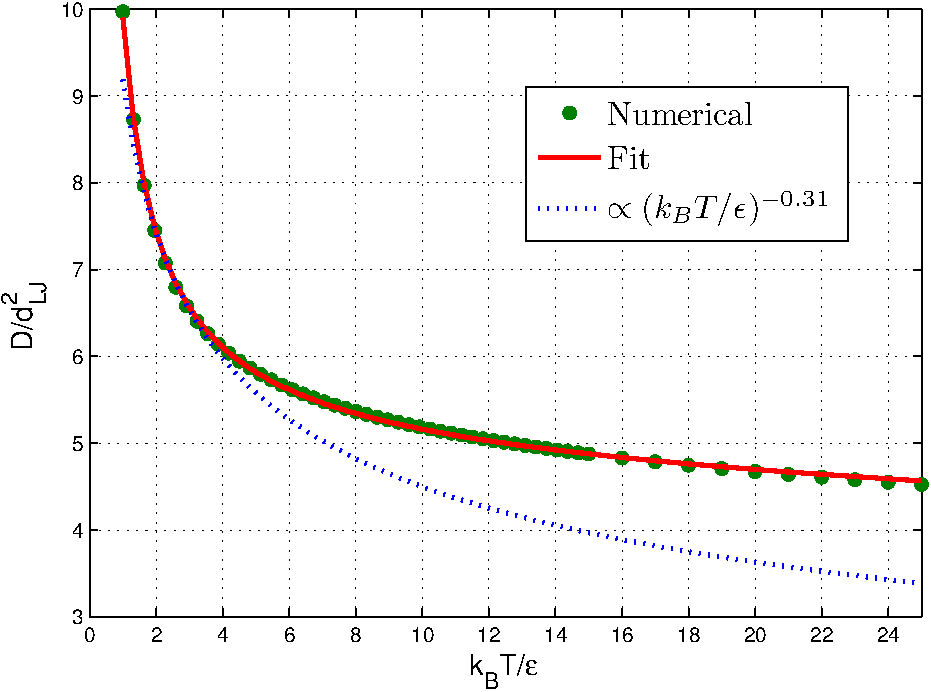
\includegraphics[scale=0.6]{Chapter4/IMG/shear_LJ3.pdf}
	\caption{
		The parameter $D$~\eqref{shear_CE_viscosity} as a function of $k_BT/\epsilon$ for the Lennard-Jones potential~\eqref{Lennard_Jones_chapter}, which is fitted by $D/d_{LJ}^2=b_1(k_BT/\epsilon)^{-0.4} +b_2(k_BT/\epsilon)^{-0.45}+b_3(k_BT/\epsilon)^{-0.5}$, where $b_1=407.4, b_2=-811.9$, and $b_3=414.4$. }
	\label{shear_LJ}
\end{figure}


For argon with the potential depth $\epsilon=119.18k_B$ in Eq.~\eqref{Lennard_Jones_chapter}, the fit in Fig.~\ref{shear_LJ} covers the temperature range from 120~K to 3000~K, while the VHS model with $\mu\propto T^{0.81}$ (dotted line) works only when 240~K$<T<$360~K. For wider temperature range, more terms with different values of $\alpha_j$ and $b_j$ may be needed. We note that, however, no matter how many terms are added (as long as $\alpha_j>-1$), the computational time of the corresponding collision operator will not increase. %The reason for this will be discussed at the end of Chapter~\ref{fourier_galerkin_spectral}. 

%In the following, if the Lennard-Jones potential is not specified, the shear viscosity of argon is proportional to $T^{0.81}$, that is, the collision kernel is given by Eq.~\eqref{kernel} or Eq.~\eqref{kernel_lei} with $\alpha=0.38$.





%\subsection{Sutherland's molecular model}
%
%For a gas whose molecules are rigid attracting spheres, i.e., the intermolecular potential is described by Eq.~\eqref{Sutherland_potential} with weak attractive fields, its shear viscosity is given by the Sutherland formula:
%\begin{equation}\label{sutherland_viscosity}
%\mu=\frac{5\sqrt{\pi{m}k_BT}}{16\sigma_{T,\infty}}\frac{T}{T+T_r},
%\end{equation} 
%where $T_r$ is a reference temperature and $\sigma_{T,\infty}$ is the total cross-section in the limiting case of infinite relative velocity $v_r$. This formula reproduces the experimental data for many real gases over a considerable range of temperature~\cite{CE,Bird1994}.
%
%
%The Sutherland formula for shear viscosity can be recovered if we use the following superposition of the modified collision kernels
%\begin{equation}\label{sutherland_kernel}
%\begin{aligned}[b]
%B=&C^{''}_{1,\gamma_1}\sin^{\gamma_1}\left(\frac{\theta}{2}\right)\cos^{-\gamma_1}\left(\frac{\theta}{2}\right)v_r\\
%+&C^{''}_{-1,\gamma_2}\sin^{\gamma_2-2}\left(\frac{\theta}{2}\right)\cos^{-\gamma_2}\left(\frac{\theta}{2}\right)v_r^{-1},
%\end{aligned}
%\end{equation}
%with the two constants ${C^{''}_{1,\gamma_1}}$ and ${C^{''}_{-1,\gamma_2}}$ satisfying
%\begin{equation}
%\begin{aligned}[b]
%8\pi{C^{''}_{1,\gamma_1}}\Gamma\left(2-\frac{\gamma_1}{2}\right)\Gamma\left(2+\frac{\gamma_1}{2}\right)=2\sigma_{T,\infty},\\
%8\pi{C^{''}_{-1,\gamma_2}}\Gamma\left(2-\frac{\gamma_2}{2}\right)\Gamma\left(1+\frac{\gamma_2}{2}\right)=2\sigma_{T,\infty}T_r\frac{4k_B}{m},\\
%\end{aligned}
%\end{equation}
%where special values of $\gamma_1$ and $\gamma_2$ (i.e., $2>\gamma_1=\gamma_2>0$) can make the FSM as fast as that for the single-term collision kernel~\eqref{kernel} or~\eqref{kernel_lei}. 



\section{Normalization}\label{Normalization_FSM}

\index{normalization}
\index{Boltzmann equation}

For practical calculations, it is convenient to introduce the following dimensionless variables:
\begin{equation}\label{normalization}
\begin{aligned}[b]
    \widetilde{f}&=\frac{v_m^3}{n_0}f, \quad
     \widetilde{\bm{x}}=\frac{\bm{x}}{L}, \quad (\widetilde{\bm{v}},\widetilde{\bm{u}},\widetilde{\bm{c}})=\frac{(\bm{v},\bm{u},\bm{c})}{v_m}, \\
\widetilde{t}&=\frac{v_m}{L}t, \quad
\widetilde{\bm{a}}=\frac{L}{v_m^2}\bm{a}, \quad
\widetilde{n}=\frac{n}{n_0}, \\
 \widetilde{T}&=\frac{T}{T_0}, \ \ \ \
\widetilde{\bm{p}}=\frac{\bm{p}}{n_0k_BT_0}, \ \ \
\widetilde{\bm{q}}=\frac{\bm{q}}{n_0k_BT_0v_m},
\end{aligned}
\end{equation}
where $n_0$ is the average number density of gas molecules, $L$ is the characteristic flow length, $v_m$ is the most probable speed at the reference temperature $T_0$. 





Under these normalization, the Boltzmann equation~\eqref{Boltzmann} with the collision kernel~\eqref{kernel_lei} takes the following form
\begin{equation}  
\label{Boltzmann_dimensionless}
\begin{aligned}
\frac{\partial \widetilde{f}}{\partial\widetilde{t}}+\widetilde{\bm{v}}\cdot\frac{\partial
\widetilde{f}}{\partial\widetilde{\bm{x}}}+\widetilde{\bm{a}}\cdot\frac{\partial
\widetilde{f}}{\partial \widetilde{\bm{v}}}=Q^+-\nu \tilde{f}.
  \end{aligned}
\end{equation}
Here, the gain term of the collision operator is  
\begin{equation}\label{coll_gain_normalization}
Q^+=\frac{1}{\text{Kn}'}\iint
\sin^{\alpha+\gamma-1}\left(\frac{\theta}{2}\right)\cos^{-\gamma}\left(\frac{\theta}{2}\right)\widetilde{v}_r^\alpha
\widetilde{f}(\widetilde{\bm{v}}'_{\ast})\widetilde{f}(\widetilde{\bm{v}}')d\Omega d\widetilde{\bm{v}}_\ast,
\end{equation}
while the loss term of the collision operator is $\nu\tilde{f}$, where the collision frequency is
\begin{equation}\label{coll_fre}
\nu=\frac{1}{\text{Kn}'}\iint
\sin^{\alpha+\gamma-1}\left(\frac{\theta}{2}\right)\cos^{-\gamma}\left(\frac{\theta}{2}\right)\widetilde{v}_r^\alpha
\widetilde{f}(\widetilde{\bm{v}}_{\ast})d\Omega d\widetilde{\bm{v}}_\ast,
\end{equation}
and 
\begin{equation}\label{Knudsen}
{\text{Kn}'}=\frac{64\sqrt{2}^\alpha}{5}\Gamma\left(\frac{\alpha+\gamma+3}{2}\right)
\Gamma\left(2-\frac{\gamma}{2}\right)\text{Kn}.
\end{equation}
It should be noted that in DSMC, the MFP of VHS model (i.e., $\lambda_{vhs}$ in Eq.~(4.52) in Ref.~\cite{Bird1994}) is frequently used. In order to compare the numerical results obtained from FSM and DSMC, the following relation should be taken into account:
\begin{equation}\label{Kn_VHS}
\begin{aligned}[b]
	%\lambda=\frac{15\pi}{2(7-2\omega)(5-2\omega)}\lambda_{VHS},	\quad\text{or}\quad 
	\text{Kn}=\frac{15\pi}{2(7-2\omega)(5-2\omega)}\text{Kn}_{vhs}.
	 \end{aligned}
\end{equation} 


\index{Lennard-Jones potential}
For the Lennard-Jones potential, when the collision kernel is approximated by Eq.~\eqref{kernel_spectral}, the term
$\sin^{\alpha+\gamma-1}(\theta/2)\cos^{-\gamma}(\theta/2){v}_r^\alpha/\text{Kn}'$
in Eqs.~\eqref{coll_gain_normalization} and~\eqref{coll_fre} should be replaced by
\begin{equation}\label{LJ_kernel}
\frac{5\sum_{j=1}^3{}b_j  (k_BT_0/2\epsilon)^{(\alpha_j-1)/2} \sin^{\alpha_j-1}({\theta}/{2})
	\widetilde{v}_r^{\alpha_j}/{\Gamma(\frac{\alpha_j+3}{2})}}
{64\sqrt{2}\text{Kn}\sum_{j=1}^3b_j(k_BT_0/\epsilon)^{(\alpha_j-1)/2}}.
\end{equation}
%A similar expression can be given for Sutherland's potential.


Considering the above normalization scheme, the normalized macroscopic quantities are related to the normalized VDF as follows:
\begin{equation}
\begin{aligned}[b]
[\widetilde{n},\widetilde{\bm{u}}, \widetilde{T}, \widetilde{p}_{ij}, \widetilde{q}_{i}]
=\int \left[1,\widetilde{\bm{v}},\frac{2}{3\widetilde{n}}\widetilde{c}^2, 2\widetilde{c}_i\widetilde{c}_j,\widetilde{c}^2\widetilde{c}_i\right]
\widetilde{f}d\widetilde{\bm{v}}.
\end{aligned}
\end{equation}
For simplicity, the tildes on normalized quantities will be omitted hereafter. 


\section{Fast spectral method}\label{single_carleman}

The numerical approximation of the Boltzmann collision operator by the FSM is introduced. For its main properties we refer to the original paper by Mouhot and Pareschi~\cite{Mouhot2006}. Detailed calculations are presented because literature gives different results for the kernel mode~\cite{Mouhot2006,Filbet2006,Hu2012}.





\subsection{Carleman representation}\label{Carleman_FSM_monatomic}
\index{Carleman representation}


We rewrite the Boltzmann collision operator using the Carleman representation. With the basic identity
\begin{equation*}
\begin{aligned}[b]
2\int_{\mathbb{R}^{3}}\delta(2\bm{y}\cdot{\bm{v}_r}+y^2)f(\bm{y})d\bm{y}=&2\int_{\mathbb{R}^{3}}\delta(|\bm{y}+\bm{v}_r|^2-v^2_r)f(\bm{y})d\bm{y}\\
=&2\int_{\mathbb{R}^{3}}\delta(y^2-v^2_r)f(\bm{y}-\bm{v}_r)d\bm{y}\\
 =&{v_r}\int_{\mathbb{S}^{2}}f(v_r\Omega-\bm{v}_r)d\Omega,
\end{aligned}
\end{equation*} 
and Eq.~\eqref{collision_velocity} for the post-collision velocities, the gain part of the collision operator~\eqref{coll_gain_normalization} is rewritten as
\begin{equation}\label{Boltzmann_gain_FSM}
\begin{aligned}[b]
 Q^+
=&\frac{1}{\text{Kn}'}\iint\Theta{v_r}
  f\left(\bm{v}_{\ast}-\frac{v_r\Omega-\bm{v}_r}{2}\right)f\left(\bm{v}+\frac{v_r\Omega-\bm{v}_r}{2}\right)d\Omega d{\bm{v}}_\ast \\
=&\frac{2}{\text{Kn}'}\iint\Theta\delta(2\bm{y}\cdot{\bm{v}_r}+y^2)
  f\left(\bm{v}_{\ast}-\frac{\bm{y}}{2}\right)f\left(\bm{v}+\frac{\bm{y}}{2}\right) d\bm{y} d{\bm{v}}_\ast \\
=&\frac{4}{\text{Kn}'}\iint\Theta\delta(\bm{y}\cdot{\bm{v}_r   }+y^2)
  f(\bm{v}_{\ast}-\bm{y})f(\bm{v}+\bm{y}) d\bm{y} d{\bm{v}}_\ast \\
=&\frac{4}{\text{Kn}'}\iint\Theta\delta(\bm{y}\cdot{}\bm{z  })
  f(\bm{v}+\bm{z})f(\bm{v}+\bm{y}) d\bm{\bm{y}} d\bm{\bm{z}},
 \end{aligned}
\end{equation}
where
$\Theta=\sin^{\alpha+\gamma-1}\left({\theta}/{2}\right)\cos^{-\gamma}\left({\theta}/{2}\right)v_r^{\alpha-1}$  if we consider the simple case where the collision kernel is given by Eq.~\eqref{kernel_lei}. Other collision kernels introduced in the above section can be handled in the same way. 


Notice that in the step-by-step calculations of Eq.~\eqref{Boltzmann_gain_FSM} we have used the transformations $\bm{y}=(v_r\Omega-\bm{v}_r)/2$ and $\bm{z}=\bm{v}_\ast-\bm{v}-\bm{y}=-\bm{v}_r-\bm{y}$; also the delta function requires that $\bm{y}$ to be perpendicular to $\bm{z}$. Therefore, the deflection angle $\theta$ satisfies 
\begin{equation}
    \cos\theta=\frac{\Omega\cdot{\bm{v}_r}}{v_r}
    =\frac{-(\bm{y}-\bm{z})\cdot(\bm{y}+\bm{z})}{|\bm{y}+\bm{z}|^2}
    \overset{\bm{y}\bot{\bm{z}}}
    {=}\frac{z^2-y^2}{y^2+z^2},
\end{equation}
which results in
\begin{equation}\label{sincos}
\begin{aligned}
\sin\left(\frac{\theta}{2}\right)=\frac{|\bm{y}|}{\sqrt{y^2+z^2}},\ \ \ \ 
\cos\left(\frac{\theta}{2}\right)=\frac{|\bm{z}|}{\sqrt{y^2+z^2}}.
\end{aligned}
\end{equation}
Hence
$\Theta=|\bm{y}|^{\alpha+\gamma-1}|\bm{z}|^{-\gamma}$ and the collision
operator is simplified to
\begin{equation}\label{ccc}
\begin{aligned}[b]
 Q=\frac{4}{\text{Kn}'}\iint&d\bm{y} d\bm{z}\delta(\bm{y}\cdot{}\bm{z})|\bm{y}|^{\alpha+\gamma-1}|\bm{z}|^{-\gamma}\\
 &\times [f(\bm{v}+\bm{z})f(\bm{v}+\bm{y})-f(\bm{v}+\bm{y}+\bm{z})f(\bm{v})].
 \end{aligned}
\end{equation}


\subsection{Fourier-Galerkin spectral method}\label{fourier_galerkin_spectral}

In FSM, the VDF is periodized on the domain $\mathcal{D}_L=[-L_v,L_v]^3$. We adopt uniform grid points in the velocity space:
\begin{equation}
v_k(j_k)=2\frac{L_v}{N_k}j_k, \quad (k=1,2,3)
\end{equation}
where $j_k\in[-N_k/2, -N_k/2+1,\cdots, N_k/2-1]$ and $N_k$ is the number of velocity grid points in the $k$-th velocity direction. Suppose $\mathcal{B}_S$, a sphere of radius $S$ centered at the origin, is the support of VDF. Usually the minimum value 
$L_v=(3+\sqrt2)S/2$ is chosen to avoid the aliasing error caused by the periodicity of VDF~\cite{Pareschi2000}. The VDF is then approximated by a truncated Fourier series,
\begin{eqnarray}
    f(\bm{v})&=&\sum_{\bm{j}=-(N_1,N_2,N_3)/2}^{(N_1,N_2,N_3)/2-1}
    \hat{f}_{\bm{j}}\exp(i\xi_{\bm{j}}\cdot{}\bm{v}), \label{fourier}\\
    \hat{f_{\bm{j}}}&=&\frac{1}{(2L_v)^3}
    \int{}f(\bm{v})\exp(-i\xi_{\bm{j}}\cdot{}\bm{v})d\bm{v},
    \label{inverse_FSM_fourier}
\end{eqnarray}
where $\xi_{\bm{j}}=\bm{j}\pi/L$ are the frequency components with $\bm{j}=(j_1,j_2,j_3)$. 


The Boltzmann collision operator~\eqref{ccc} is also truncated, with the infinite velocity space replaced by the finite one in ${\mathcal{B}_R}$, where the truncation radius $R$ satisfies~\cite{Mouhot2006,Filbet2006}:
\begin{equation}\label{velocity_truncation}
R\ge\sqrt{2}S.
\end{equation} 
Numerical analysis in Fig.~\ref{test_R} will show that, however, $R$ cannot be larger than $L$. Expanding the truncated collision operator by Fourier series, we find that the $\bm{j}$-th spectrum of the truncated collision operator is related to spectrum $\hat{f}$ as:
\begin{equation}\label{mo_monatomic_de}
   \widehat{Q}_{\bm{j}}= \sum_{\bm{l}+\bm{m}=\bm{j} \atop
    \bm{l},\bm{m}=-(N_1,N_2,N_3)/2}^{{(N_1,N_2,N_3)}/2-1}\hat{f}_{\bm{l}}\hat{f}_{\bm{m}}[\beta(\bm{l},\bm{m})-\beta(\bm{m},\bm{m})],
\end{equation}
where $\bm{l}=(l_1,l_2,l_3)$, $\bm{m}=(m_1,m_2,m_3)$, and the kernel mode
$\beta(\bm{l},\bm{m})$ is simplified to 
\begin{equation}\label{kernel_FSM_mode0}
\begin{aligned}[b]
\beta(\bm{l},\bm{m})=&\frac{4}{\text{Kn}'}\iint
\delta(\bm{y}\cdot{\bm{z}})|\bm{y}|^{\alpha+\gamma-1}|\bm{z}|^{-\gamma}
\exp(i\xi_{\bm{l}}\cdot{\bm{y}}+i\xi_{\bm{m}}\cdot{\bm{z}})d\bm{y}d\bm{z}\\
   =&\frac{1}{\text{Kn}'}\int\int \delta(\bm{e}\cdot{\bm{e}'})
              \left[\int_{-R}^R|\rho|^{\alpha+\gamma}\exp(i\rho\xi_{\bm{l}}\cdot{\bm{e}})d\rho\right]\\
              &\ \ \ \ \ \ \ \ \ \ \ \ \ \ \ \ \ \ \ \ \times\left[\int_{-R}^R|\rho'|^{1-\gamma}\exp(i\rho'\xi_{\bm{m}}\cdot{\bm{e}'})d\rho'\right]d\bm{e}'d\bm{e} \\
=&\frac{1}{\text{Kn}'}\int_{\mathbb{S}^2}
    \phi_{\alpha+\gamma}(\xi_{\bm{l}}\cdot{\bm{e}})
    \left[\int_{\mathbb{S}^2}\delta(\bm{e}\cdot{\bm{e}'})\phi_{1-\gamma}(\xi_{\bm{m}}\cdot{}\bm{e}')d\bm{e}'\right]d\bm{e},
\end{aligned}
\end{equation}
with $\bm{e}, \bm{e}'$ being the unit vectors in the sphere $\mathbb{S}^{2}$, and
\begin{equation}\label{phi_FSM_expression}
    \phi_\delta(s)=2\int_{0}^R\rho^\delta\cos\left(\rho{s}\right)d\rho.
\end{equation}


\begin{figure}[t]
	\centering
	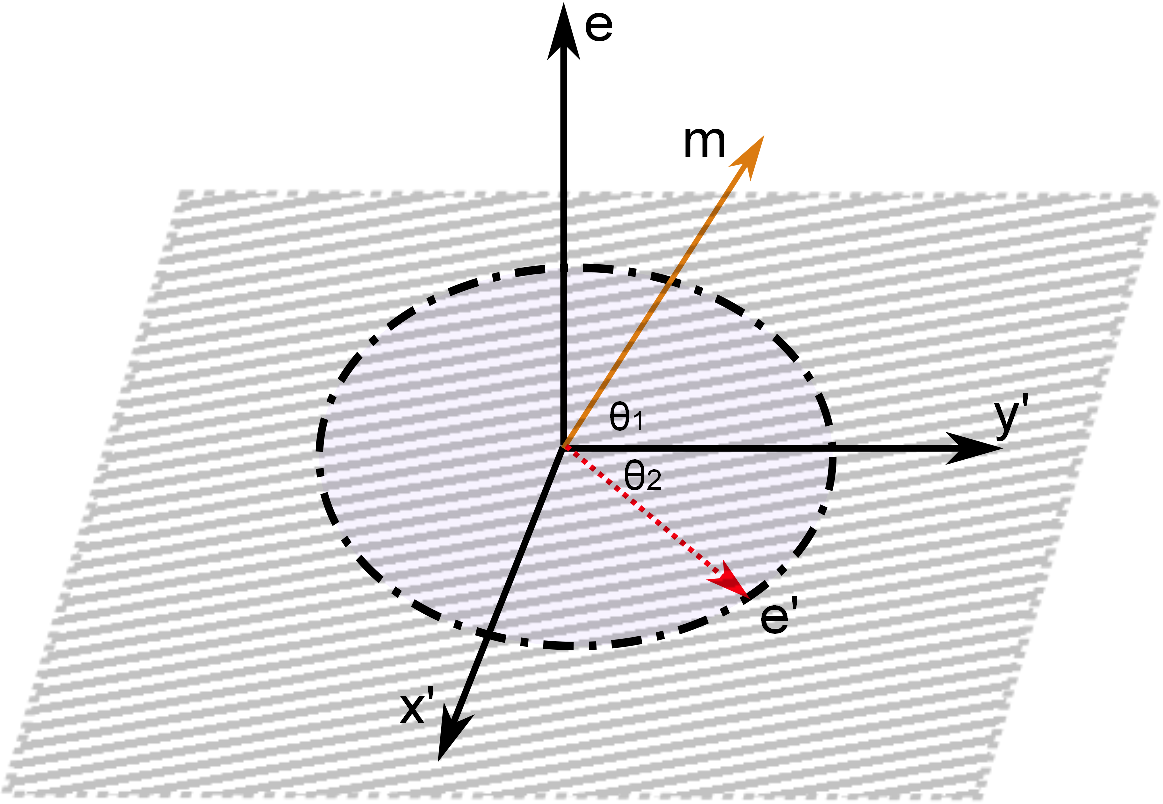
\includegraphics[width=7.5cm]{Chapter4/IMG/demo.pdf}
	\caption{
		Demonstration of the integral with respect to $\bm{e}'$ used in the calculation of kernel mode~\eqref{kernel_FSM_mode0}. When the vector $\bm{e}$ is fixed, we can make the $x'y'$ plane perpendicular to $\bm{e}$ and $m$ fall in the $ey'$ plane. The vector $\bm{e}'$ degenerates to a two-dimensional vector characterized by the polar angle $\theta_2$ varying from 0 to $2\pi$. The polar and azimuthal angles of $\bm{e}'$ in the new coordinate system are $\theta$ and $\pi/2-\theta_2$, respectively, and the angle between the vector $\bm{m}$ and $y'$-axis is $\theta_1$. 
	} 
	\label{demo}
\end{figure}


Equation~\eqref{kernel_FSM_mode0} can be simplified further. We construct a new Cartesian coordinate system, where its ${z}'$ axis is parallel to $\bm{e}$, the $y'$ axis is just the projection of vector $\bm{m}$ into the plane $e_\bot$ perpendicular to the $z'$ axis, and the $x'$ axis is in the plane $e_\bot$ and perpendicular to the $y'$ axis, see Fig.~\ref{demo}. Suppose the polar and azimuthal angles of $\bm{e}'$ in the new coordinate system are $\theta$ and $\pi/2-\theta_2$, respectively, and the angle between the vector $\bm{m}$ and $y'$-axis is $\theta_1$. Then, we have $\delta(\bm{e}\cdot{\bm{e}'})=\delta(\cos\theta)$ so that $\int_0^\pi g(\theta)\delta(\cos\theta)d\theta=g(\pi/2)$ for smooth function $g(\theta)$, $\xi_{\bm{m}}\cdot{}\bm{e}'=|\xi_{\bm{m}}|\cos\theta_1\cos\theta_2$, and the kernel mode becomes
\begin{equation}\label{kernel_mode2}
\begin{aligned}[b]
\beta(\textbf{l},\textbf{m})&=\frac{1}{\text{Kn}'}\int_{\mathcal{S}^2}d\textbf{e} \phi_{\alpha+\gamma}(\xi_\textbf{l}\cdot{\textbf{e}}) \\
&\times
\left[\int_0^{2\pi}\int_0^\pi\delta(\cos\theta)\phi_{1-\gamma}(|\xi_\textbf{m}|
\cos\theta_{1}\cos\theta_2)d\theta{d\theta_2}\right]\\
&=\frac{1}{\text{Kn}'}\int_{\mathcal{S}^2}\phi_{\alpha+\gamma}(\xi_\textbf{l}\cdot{\textbf{e}})
\left[\int_0^{2\pi} \phi_{1-\gamma}(|\xi_\textbf{m}|\cos\theta_1\cos\theta_2)d\theta_2\right]d\textbf{e}\\
&=\frac{2}{\text{Kn}'}\int_{\mathcal{S}^2}\phi_{\alpha+\gamma}(\xi_\textbf{l}\cdot{\textbf{e}})
\cdot\psi_{\gamma}(|\xi_\textbf{m}|\cos\theta_1)d\textbf{e},
\end{aligned}
\end{equation}
%\begin{equation}\label{kernel_mode2}
%\begin{aligned}[b]
%\beta(\bm{l},\bm{m})
%        &=\frac{1}{\text{Kn}'}\int_{\mathcal{S}^2}\phi_{\alpha+\gamma}(\xi_{\bm{l}}\cdot{\bm{e}})
%\left[\int_0^{2\pi} \phi_{1-\gamma}(|\xi_{\bm{m}}|\cos\theta_1\cos\theta_2)d\theta_2\right]d\bm{e}\\
%        &=\frac{2}{\text{Kn}'}\int_{\mathcal{S}^2}\phi_{\alpha+\gamma}(\xi_{\bm{l}}\cdot{\bm{e}})
%                \cdot\psi_{\gamma}(|\xi_{\bm{m}}|\cos\theta_1)d\bm{e},
%\end{aligned}
%\end{equation}
where
\begin{equation}\label{psi_FSM_expression}
 \psi_{\gamma}(s)=\int_0^\pi\phi_{1-\gamma}(s\cos\theta_2)d\theta_2=2\pi\int_0^R \rho^{1-\gamma} J_0(\rho s)d\rho, %=2\pi{R}\frac{J_1(Rs)}{s},
\end{equation}
with $J_0$ being the zeroth-order Bessel function.


Note that $\xi_{\bm{l}}$ and $\xi_{\bm{m}}$ in Eq.~\eqref{kernel_mode2} appear in two functions. If they also appear in two different functions in the final form of $\beta(\bm{l},\bm{m})$, Eq.~\eqref{mo_monatomic_de} can be calculated effectively by the FFT-based convolution. The separation of $\bm{l}$ and $\bm{m}$ in Eq.~\eqref{kernel_mode2} can be realized approximately using the numerical quadrature. Two different methods will be employed and compared:
\begin{itemize}
    \item  in the first method, $\beta(\bm{l},\bm{m})$ is calculated numerically in spherical coordinates by the trapezoidal rule. Suppose the polar and azimuthal angles of the unit vector $\bm{e}$ are $\theta$ and $\varphi$, respectively. We divide each region $0\le\theta\le\pi$ and $0\le\varphi\le\pi$ (for symmetry) into $M$ sections: $\theta_p=p\pi/M$ and $\varphi_q=q\pi/M$ with $p,q=1,2,\cdots,M$. Then the kernel mode~\eqref{kernel_mode2} is approximated by
    \begin{equation}\label{kernel_FSM_mode}
    \begin{aligned}[b]
    \beta(\bm{l},\bm{m})\simeq\frac{4\pi^2}{\text{Kn}'M^2}\sum_{p,q=1}^{M-1,M}
    \phi_{\alpha+\gamma}(\xi_{\bm{l}}\cdot{\bm{e}_{\theta_p,\varphi_q}})
        \psi_{\gamma}(\xi^\perp_{\bm{l}})
        \cdot\sin\theta_p,
        \end{aligned}
    \end{equation}
    where 
    \begin{equation}
    \xi^\perp_{\bm{l}}=\sqrt{|\xi_{\bm{m}}|^2-(\xi_{\bm{m}}\cdot{\bm{e}}_{\theta_p,\varphi_q})^2}.
    \end{equation}
           
    \item  in the second method, $\beta(\bm{l},\bm{m})$ is approximated by a  Gauss-Legendre quadrature of order $M$ (see the Matlab code in Appendix~\ref{appen_GaussLegendre}):
    \begin{equation} \label{kernel_FSM_modee}
    \begin{aligned}[b]
    \beta(\bm{l},\bm{m})\simeq\frac{4}{\text{Kn}'}\sum_{p,q=1}^{M}{\omega_p\omega_q}
    \phi_{\alpha+\gamma}(\xi_{\bm{l}}\cdot{\bm{e}_{\theta_p,\varphi_q}})\psi_{\gamma}(\xi^\perp_{\bm{l}})\cdot\sin\theta_p,
        \end{aligned}
    \end{equation}
            where $\theta_p\ (\varphi_q)$ and $\omega_p\  (\omega_q)$ are the $p\ (q)$-th point and weight in the Gauss-Legendre quadrature with  $\theta, \varphi\in[0,\pi]$, and the unit vector is expressed as
            \begin{equation}
           \bm{e}_{\theta_p,\varphi_q}=(\sin\theta_p\cos\varphi_q,\sin\theta_p\sin\varphi_q,\cos\theta_p).
            \end{equation}
\end{itemize}

\begin{figure}[t]
	\centering
	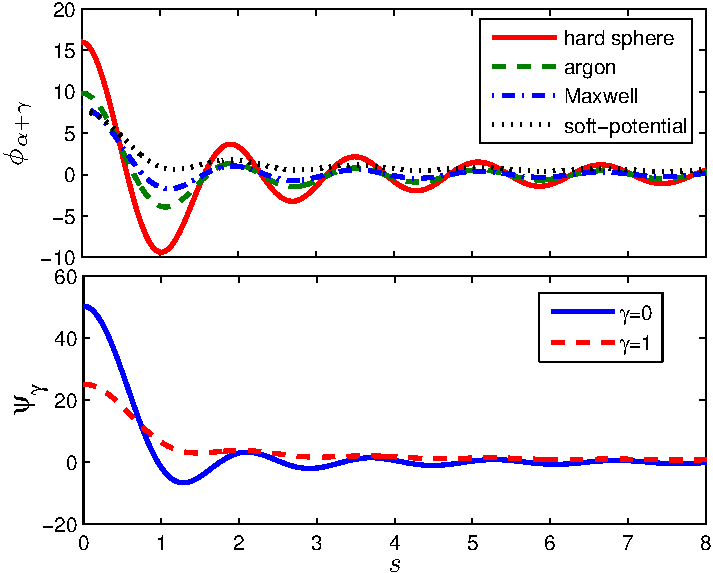
\includegraphics[width=10cm]{Chapter4/IMG/phi_psi2.pdf}
	\caption{
		Profiles of $\phi_{\alpha+\gamma}$  and $\psi_\gamma$ according to Eqs.~\eqref{phi_FSM_expression} and~\eqref{psi_FSM_expression} when $R=4$ and $\gamma=0$. Because of symmetry, the region $s<0$ is not plotted. For the soft potential, we use $\alpha=-0.4$ and the shear viscosity is proportional to $T^{1.2}$.
	}
	\label{phi_psi}
\end{figure}

The analytical form of $\phi_{\alpha+\gamma}(s)$ can be obtained when $\alpha+\gamma$ is an integer. For instance, when $\gamma=0$, for Maxwell molecules $(\alpha=0)$ and HS $(\alpha=1)$ molecules, we have
\begin{equation}\label{int_res}
  \begin{aligned}[b]
    \phi_0(s)=\frac{2\sin(Rs)}{s},\\
    \phi_1(s)=\frac{2R\sin(Rs)}{s}-\frac{4\sin^2(Rs/2)}{s^2},
  \end{aligned}
\end{equation}
while for  other cases $\phi_{\alpha+\gamma}(s)$ and $\psi_{\gamma}(s)$ can be accurately calculated by Gauss-Legendre quadrature numerically. Fig.~\ref{phi_psi} shows typical decaying-oscillating profiles of the two functions $\phi_{\alpha+\gamma}$ and $\psi_\gamma$, where  the quasi-period of oscillation is about $2\pi/R$.




Note that in the VHS model, $-3<\alpha\le1$. From Eq.~\eqref{phi_FSM_expression} it follows that $\delta$ is restricted to the region $(-1,+\infty)$. Therefore, $\alpha+\gamma>-1$ and $1-\gamma>-1$. In the original collision kernel proposed by Mouhot and Pareschi~\cite{Mouhot2006}, $\gamma=0$, so that $\alpha$ is restricted in the region $(-1,1]$. This means that the original collision kernel cannot deal with general forms of soft potentials. In our modified collision kernel~\eqref{kernel_lei}, if we let $\gamma\rightarrow2$, $\alpha$ can cover the whole region $(-3,1]$, thus extending the applicability of FSM to all inverse power-law potentials except the Coulomb potential. 


It should also be noted that for the Lennard-Jones potential, the storage of the kernel modes and computational cost of the collision operator is exactly the same as that for the single-term collision kernel~\eqref{kernel} or~\eqref{kernel_lei}. 
%For the collision kernel~\eqref{sutherland_kernel} of the Sutherland potential, if we let $\gamma_1=\gamma_2$, the storage and computational cost will also be the same as the single-term collision kernel. 
For the existence of $\phi_{1+\gamma_1}$, $\psi_{1-\gamma_1}$, $\phi_{-1+\gamma_2}$, and $\psi_{1-\gamma_2}$, one should choose $-2<\gamma_1<2$ and $0<\gamma_2<2$. Therefore, we choose $0<\gamma_1=\gamma_2<2$. If $\gamma_1\neq\gamma_2$, the storage and computational cost will be twice of that of the single-term collision kernel~\eqref{kernel_lei}.


\subsection{Detailed implementation}

The detailed procedure to calculate the Boltzmann collision operator is now outlined. Let us assume Eq.~\eqref{kernel_mode2} is approximated by the trapezoidal rule. First, the kernel modes is pre-computed and stored. The storage of $\phi_{\alpha+\gamma}(\xi_{\bm{l}},\theta_p,\varphi_q)$ and $\psi_{\gamma}(\xi_{\bm{m}},\theta_p,\varphi_q)$ requires $2M(M-1)N_1N_2N_3$ units of compute memory. We also need $N_1N_2N_3$ units of storage for
\begin{equation}\label{phi_loss}
\phi_{loss}=\sum_{p,q=1}^{M-1,M}\phi_{\alpha+\gamma}(\xi_{\bm{m}},\theta_p,\varphi_q)
    \psi_{\gamma}(\xi_{\bm{m}},\theta_p,\varphi_q)\sin\theta_p,
\end{equation}
which is used to calculate the collision frequency in Eq.~\eqref{coll_fre}. For space-homogeneous problems, such storage is relatively large when compared to the storage of VDF. However, when it comes to space-inhomogeneous problems, the storage will be relatively small because different spatial grids share the same kernel modes. 


\begin{figure}[t]
	\centering
	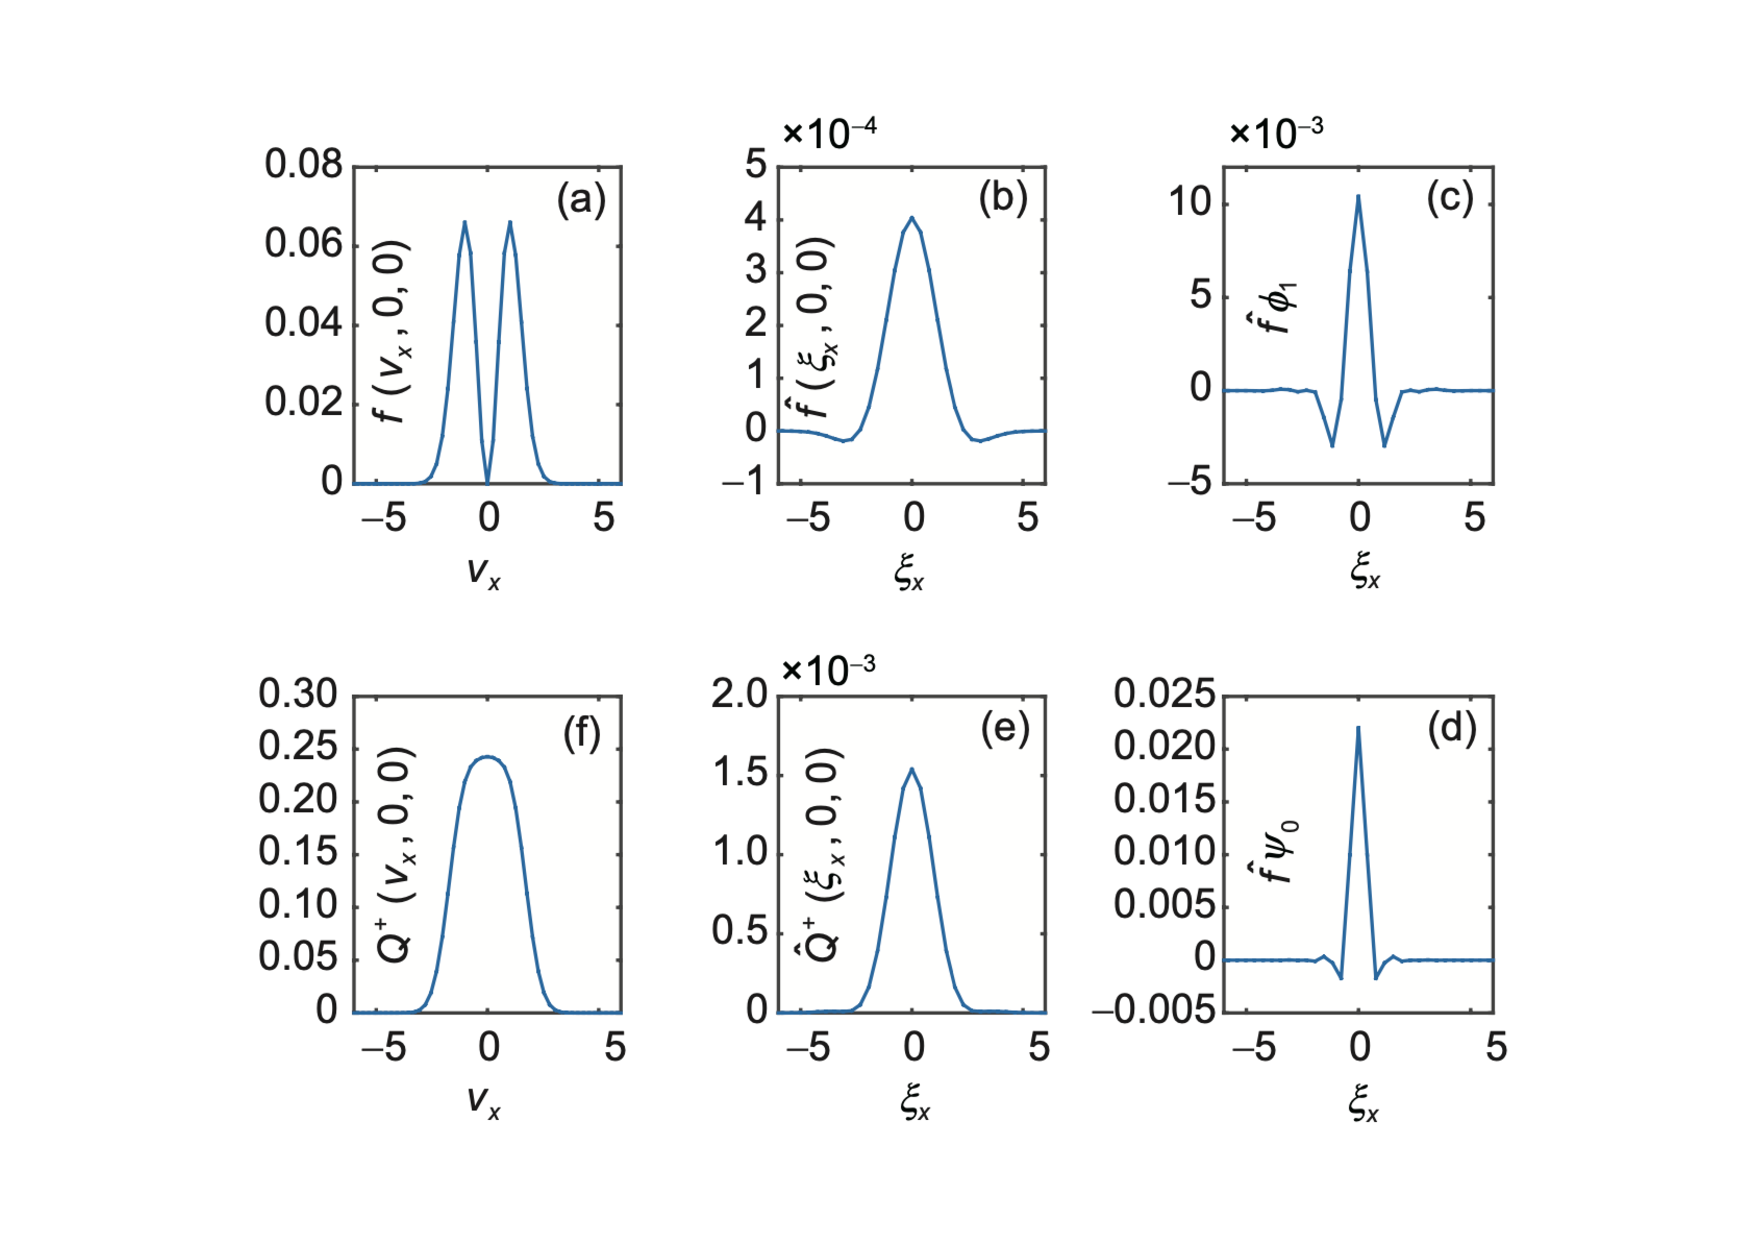
\includegraphics[scale=0.5]{Chapter4/IMG/FSM_demo.pdf}
	\caption{
		Numerical implementation of the FSM for the gain part of Boltzmann collision operator~\eqref{coll_gain_normalization}. Given the VDF in (a), its spectrum in obtained in (b) by inverse FFT. Then the spectrum is respectively multiplied with the kernel modes $\phi$ and $\psi$ (the results are in (c) and (d), respectively), and their convolution is shown in (e). The FFT of (e) gives the gain part of the Boltzmann collision operator for specific combination of $p$ and $q$ in (f). Summering $Q^+$ for all combinations of $p$ and $q$ gives the gain part of the Boltzmann collision operator. Note that the whole process is done in three-dimensional velocity space and spectrum space, but for clarity only the one-dimensional results are shown.
	  }
	\label{FSM_demo}
\end{figure}


Second, we obtain the spectrum of VDF by applying the inverse FFT to $f$. Then, with Eq.~\eqref{kernel_FSM_mode}, Eq.~\eqref{mo_monatomic_de} becomes 
\begin{equation*}
\begin{aligned}[b]
  \widehat{Q}_{\bm{j}}\approx &\underbrace{\frac{4\pi^2}{\text{Kn}'M^2}\sum_{p,q=1}^{M-1,M} \sum_{\bm{l}+\bm{m}=\bm{j} }[\hat{f}_{\bm{l}}{\phi_{\alpha+\gamma}(\xi_{\bm{l}},\theta_p,\varphi_q)}]\cdot[\hat{f}_{\bm{m}}{\psi_{\gamma}(\xi_{\bm{m}},\theta_p,\varphi_q)}]}_{gain}\cdot\sin\theta_p
  \\
  &\underbrace{-\frac{4\pi^2}{\text{Kn}'M^2}\sum_{\bm{l}+\bm{m}=\bm{j} }\hat{f}_{\bm{l}}\cdot[\hat{f}_{\bm{m}}{\phi_{loss}}]}_{loss}.
\end{aligned}
\end{equation*}

The loss term can be effectively calculated by FFT-based convolution, using the zero-padding technique~\cite{Canuto1998}. For the gain term, one has to do FFT-based convolution for each pair of $(p,q)$, that is, $M(M-1)$ times. The implementation is listed in Steps 2, 3, and 4 in the algorithm 1 of Appendix~\ref{appen_FSM}. Finally, the collision operator $Q$ is calculated by applying the FFT to $\widehat{Q}$ (Step 5). The whole process is visualized in Fig.~\ref{FSM_demo}.

Note that in algorithm 1 the zero-padding technique is employed to eliminate the aliasing error in FFT-based convolution. This process is accurate for arbitrary values of $t_1$ and $t_2$ (defined in Appendix~\ref{appen_FSM}) when the padding size in each direction is larger than one half of the velocity grid number. Considering the fact that the spectrum $\hat{f}$ is non-zero only in the central region of frequency domain, we can expedite the calculation by ignoring zero-padding. This leads to the simpler and faster algorithm 2: numerical simulations show that both algorithms produce identical results, but the algorithm 2 is about 4 times faster than the algorithm 1.


Now we see that the computational cost of FSM is $O(M^2N^3\log{}N)$, where $N$ is the same order as $N_1,N_2$ and $N_3$. Note that $\bm{l}$ and $\bm{m}$ are not separable in classical spectral methods, and the computational cost of Eq.~\eqref{mo_monatomic_de} is $O(N^6)$~\cite{Gamba2009,Pareschi2000}. A rough estimate of the speed-up can be given. In algorithm 2, one needs to do $2M(M-1)+2$ times FFT (the array size is $N_1\times{N_2}\times{N_3}$), while in classical spectral methods the computational cost is the same with one direct convolution of one complex and one real array of size $N_1\times{N_2}\times{N_3}$. For comparison, we take $M=7$ and run our Matlab (version 2012a) programs on a PC with an Intel Xeon 3.3 GHz CPU. For $N=32$ (or 64), algorithm 2 is about 18 (or 62) times faster than the classical spectral methods. Further speed-up can be achieved by reducing the value of $M$, say, to 5. 

%As will shown in Chapter~\ref{chap:linearized}, for the flows with large Knudsen number there are discontinuities in the VDF; to capture the discontinuities, one needs large number of velocity grids. In this case, the FSM could be faster than the classical spectral methods by two orders of magnitude. 


\subsubsection{Conservation enforcement}%\label{conservation_single}

One of the drawbacks of FSM, as with any spectral methods in the approximation of Boltzmann collision operator, is that it does not exactly conserve the momentum and energy. To ensure the conservation of momentum and energy, the method of Lagrangian multipliers can be employed~\cite{Gamba2009}: after the collision operator $Q$ is approximated, we construct $Q^{new}$ by minimizing the function $\sum_{\bm{j}}(Q_{\bm{j}}-Q_{\bm{j}}^{new})^2$ under the constraints $\sum_{\bm{j}} Q_{\bm{j}}^{new}=\sum_{\bm{j}} \bm{v}Q_{\bm{j}}^{new}=\sum_j {v^2}Q_{\bm{j}}^{new}=0$, yielding
\begin{equation*}\label{Lagrangian1}
{Q}^{new}={Q}-(\lambda_n+\lambda_{\bm{v}}\cdot{}\bm{v}+\lambda_e {v^2}),
\end{equation*}
where the five Lagrangian multipliers satisfy
\begin{equation*}
\begin{aligned}[b]
\sum_{\bm{j}} Q=\sum_j (\lambda_n+\lambda_{\bm{v}}\cdot{}\bm{v}+\lambda_e |\bm{\bm{v}}|^2), \\
\sum_{\bm{j}} \bm{v}Q=\sum_j \bm{v}(\lambda_n+\lambda_{\bm{v}}\cdot{}\bm{v}+\lambda_e {v^2}), \\
\sum_{\bm{j}} {v^2} Q=\sum_j {v^2}(\lambda_n+\lambda_{\bm{v}}\cdot{}\bm{v}+\lambda_e {v^2}).
\end{aligned}
\end{equation*}

Since the errors for the momentum and energy in FSM are spectrally small~\cite{Mouhot2006}, the Lagrangian multipliers are very small. In practice, we normally do not use  conservation enforcement if the steady-state solution of the Boltzmann equation can be quickly found.



\subsection{Non-uniform discretization of velocity space}

In the simulation of rarefied gas flows with large Knudsen numbers, the ``over concentration'' phenomenon are frequently encountered~\cite{Takata2011}, where the VDF concentrates or has sharp variations around $v\sim0$ due to the wall effect. To tackle this problem, the molecular velocity space should be discretized non-uniformly, with more points placed near $v=0$. In microflows, we usually use the following non-uniform discretization:
\begin{equation}\label{nonuniform_v}
v_i=\frac{L_v}{(N_v-1)^\imath}(-N_v+1,-N_v+3,\cdots,{N_v-1})^\imath,
\end{equation}
where $\imath$ is a positive odd number, $L_v$ is the velocity bound, and $N_v$ is the total number of discretized velocity in the $i$-th direction. 


However, the frequency space must be discretized uniformly, otherwise the FFT-based convolution cannot be applied efficiently. This means that Steps 2 and 3 in the algorithm of Appendix~\ref{appen_FSM} remain unchanged, but the Fourier transform in Steps 1 and 4 is calculated by direct summation. Fortunately, the computational cost can be reduced by considering the following two factors:
\begin{itemize}
	\item the number of discretized frequency components $N_\xi$ can be different from the corresponding velocity components $N_v$. In fact, $N_\xi$ can be much smaller than $N_v$ due to the spectral accuracy of FSM; hence the computational cost of the convolution is $O(M^2N_{\xi}\ln{N_{\xi}})$.
	
	\item in the rectangular Cartesian coordinates, the Fourier transform in Steps 1 and 4 can be done by direct summation in each direction sequentially, thus the cost will be at the order of $N_v^3N_\xi\ln{}N_v$. This cost is certainly higher than the FFT on uniform grids, but is only comparable to the FFT-based convolution in Steps 2 and 3. 
\end{itemize}
Therefore, compared to the uniform discretization with large number of velocity grids, the use of non-uniform velocity grids will not only reduce computational memory, but also computational time.

%The number of frequency components in the $\xi_1$ and $\xi_3$ directions are $N_1'N_3'=24\times24$, and there are $N_2'$ frequency components in the $\xi_2$ direction. The FFT is used in the $v_1$ and $v_3$ directions, while in the $v_2$ direction the direct sum is implemented: for nonuniform velocity grids~\eqref{nonuniform_v}, we use $\sum_m{}g(v_{2m})w_m$ to approximate  $\int{}g(v_2)dv_2$, where 

%\begin{equation}
%w_m=\imath{}L(-N_2+1,-N_2+3,\cdots,{N_2-1})^{\imath-1}/(N_2-1)^\imath.
%\end{equation}
%The resulting  overall computational cost is $O(N_2N_2'N_1'N_3'\ln(N_1'N_3'))$, which is comparable to the FFT-based convolution sum of equation~\eqref{detailed_linear_half}. 
%
%
%The calculation of $\mathcal{L}_g(h^k)$ is as follows: when $h^k$ is known, we obtain $\hat{\mathcal{L}}_g$ from equation~\eqref{detailed_linear_half}. Then we obtain $\mathcal{L}_g(h^k)$ by applying the inverse FFT to $\hat{\mathcal{L}}_g$:
%$
%\mathcal{L}_g(h^k)=\sum_{\textbf{j}=-\textbf{N}/2}^{\textbf{N}/2-1}\hat{\mathcal{L}}_g(j)\exp(i\xi_\textbf{j}\cdot{}\textbf{v})
%$. 





\section{Accuracy in homogeneous relaxation}
\index{homogeneous relaxation}

To assess the accuracy of FSM, the relax-to-equilibrium process of Maxwell molecules ($\alpha,\gamma=0$) is considered. This is a spatial-homogeneous problem, where the Boltzmann equation becomes 
\begin{eqnarray}
 \frac{\partial {f}}{\partial{t}}=\frac{1}{\text{Kn}'}\iint
\sin^{-1}\left(\frac{\theta}{2}\right)
[{f}({\bm{v}}'_{\ast}){f}({\bm{v}}')-{f}({\bm{v}}_\ast)
  {f}({\bm{v}})]d\Omega d{\bm{v}}_\ast. 
  \label{Boltzmann_homogeneous}
\end{eqnarray}
Without loss of generality, we choose $\text{Kn}'=32\pi/5$. And for simplicity we consider the uniform discretization of molecular velocity space.

\subsection{Bobylev-Krook-Wu solution}
\index{Bobylev-Krook-Wu}

Equation~\eqref{Boltzmann_homogeneous} possesses the exact Bobylev-Krook-Wu (BKW) solution~\cite{BKW}:
\begin{equation}\label{initial_2}
    f(\bm{v},t)=\frac{1}{2(2\pi{K})^{3/2}}\exp\left(-\frac{{v^2}}{2K}\right)\left(\frac{5K-3}{K}+\frac{1-K}{K^2}{v^2}\right),
\end{equation}
where  $K=1-0.4\exp\left(-{t}/{6}\right)$. The evolution of the fourth- and sixth-order moments is given by
\begin{equation}\label{initial_22}
\begin{aligned}[b]
	M_4=\int fv_1^4d\bm{v}=6K-3K^2,\\ 
	M_6=\int fv_1^6d\bm{v}=45K^2-30K^3.
\end{aligned}
\end{equation}


\begin{table}[t]
	\centering
	\caption[Relative error in the approximation of the Boltzmann collision operator.]{Relative error $\sum_{\bm{j}}|Q_{\bm{j}}^{nu}-Q_{\bm{j}}^{an}|/\sum_{\bm{j}}|Q_{\bm{j}}^{an}|$ in the approximation of the Boltzmann collision operator. T (G) stands for the trapezoidal (Gauss-Legendre) quadrature used in the approximation of Eq.~\eqref{kernel_mode2}. Parameters are $L=8$ and $R=6$. } \label{table_coll} 
		\begin{tabular}{ccccccccccccccc}
			\hline
			N  &    & $M=5$    & 6       & 7        & 8         & 12       & 16       \\
			$16$& T  & 4.58E-1  & 4.73E-1 & 4.55E-1  & 4.52E-1   & 4.78E-1   & 4.83E-1  \\
			& G  & 2.10E-1  & 3.35E-1 & 2.48E-1  & 2.77E-1   & 2.74E-1   & 2.69E-1  \\
			24 & T  & 7.94E-2  & 5.20E-2 & 4.73E-2  & 3.93E-2   & 2.92E-2   & 2.59E-2  \\
			& G  & 4.61E-2  & 2.09E-2 & 9.16E-3  & 2.10E-2   & 1.72E-2   & 1.37E-2  \\
			32 & T  & 5.54E-2  & 3.51E-2 & 2.57E-2  & 1.93E-2   & 8.39E-3   & 4.75E-3  \\
			& G  & 4.26E-2  & 6.18E-3 & 6.49E-4  & 2.11E-4   & 1.86E-4   & 1.57E-4  \\
			48 & T  & 4.26E-2  & 3.88E-2 & 2.77E-2  & 2.08E-2   & 8.99E-3   & 5.01E-3  \\
			& G  & 4.31E-2  & 6.17E-3 & 6.09E-4  & 4.56E-5   & 4.94E-6   & 3.85E-6  \\
			64 & T  & 5.90E-2  & 3.87E-2 & 2.77E-2  & 2.08E-2   & 8.99E-3   & 5.02E-3  \\
			& G  & 4.30E-2  & 6.16E-3 & 6.10E-4  & 4.70E-5   & 3.87E-6   & 4.31E-6  \\
			\hline
		\end{tabular}
	\end{table}


\begin{figure}[t]
	\centering
	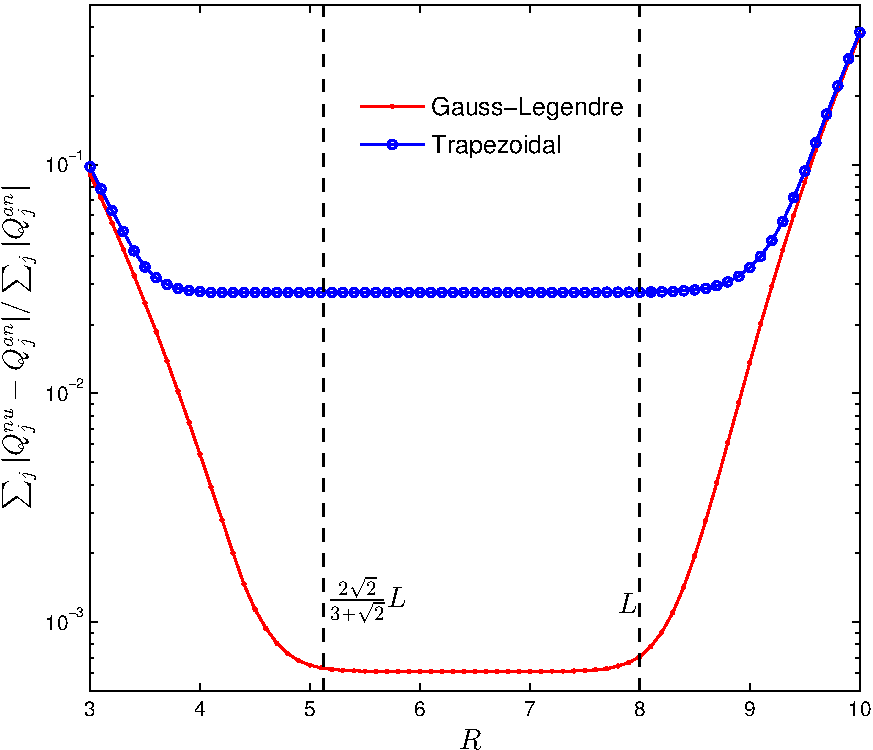
\includegraphics[width=7.5cm]{Chapter4/IMG/error_coll.pdf}
	\caption{
		The relative error versus the truncation radius $R$. Parameters are $L=8, N=48$, and $M=7$. The Gauss-Legendre quadrature is used in the approximation of the kernel mode.
	}
	\label{test_R}
\end{figure}


The integration of Eq.~\eqref{Boltzmann_homogeneous} with respect to $t$ will introduce some numerical error. In order to assess how accurately the FSM can approximate the Boltzmann collision operator, we compare $Q^{nu}$, the numerical approximation of $Q$, to the analytical solution $Q^{an}$, which is calculated by
\begin{equation}
Q^{an}(\bm{v})=\frac{f(\Delta{t},\bm{v})-f(0,\bm{v})}{\Delta{t}},
\end{equation}
with $\Delta{t}$=1.0E-5 (which is far smaller than the characteristic relaxation time $\text{Kn}'$). The following two factors affect the accuracy:
\begin{itemize}
	\item $N$, which decides the accuracy of the spectrum $\hat{f}$ of VDF;
	\item $M$, which determines how accurately we approximate Eq.~\eqref{kernel_mode2}.
\end{itemize}

The influence of $M$ is analyzed as follows. For simplicity, let us ignore $\xi_{\bm{m}}$ and $\varphi$ in Eq.~\eqref{kernel_mode2}. Notice that $\phi_{\alpha+\gamma}$ is a decaying-oscillating function with the quasi-period $2\pi/R$ (see Eq.~\eqref{int_res} and Fig.~\ref{phi_psi}). Then, for a fixed value of $\xi_{\bm{l}}$, the integral kernel in Eq.~\eqref{kernel_mode2} oscillates $R|\xi_{\bm{l}}|/\pi$ times as $\theta$ varies from 0 to $\pi$. In the worst case ($\xi_{\bm{l}}\rightarrow{}N\pi/2L$), it oscillates $O(N)$ times. This implies that $M$ should be $O(N)$. In practical calculations, however, $M$ can be far less than $N$ because, if the VDF has a support $S$, its spectrum has a support $1/S\sim{1/R}$. Within this support, the integral kernel in Eq.~\eqref{kernel_mode2} oscillates only a few times, and hence a small value of $M$ can lead to accurate result.


\begin{figure}[t]
	\centering
	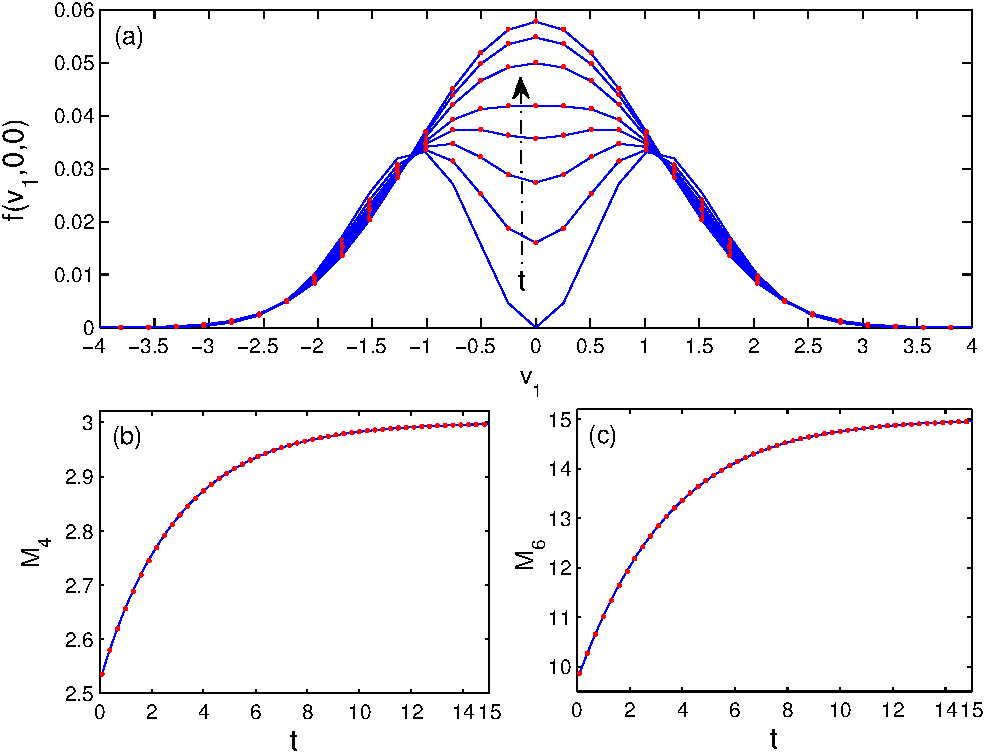
\includegraphics[width=11cm]{Chapter4/IMG/test11.pdf}
	\caption{
		(a) Evolution of $f(v_1,0,0)$ of space-homogeneous Maxwell molecules, from the initial condition~\eqref{initial_2}. From bottom to top (near $v_1=0$), the time corresponding to each line is $0, 0.5, 1, 1.5, 2, 3, 4$, and $5$. (b) and (c) Evolution of the fourth- and sixth-order moments, respectively. Solid lines: numerical result. Dots: analytical solution. Other parameters used in the numerical simulation are: $L=8, R=6$, $N=64$, and $M=5$ with Eq.~\eqref{kernel_FSM_mode}.  
	}
	\label{test2}
\end{figure}



We vary the values of $N$ and $M$ to see their influence on the numerical accuracy; the results are tabulated in Table~\ref{table_coll}. When $N=16$, the relative error is large because the resolution of VDF is not high enough so that a large error exists in the spectrum $\hat{f}$. As $N$ increases to 24, the error is reduced by one order of magnitude. When the trapezoidal rule is used, the error mainly comes from the approximation of Eq.~\eqref{kernel_mode2}, which decays at $O(M^{-2})$ when $N$ is fixed. When $M$ is fixed, the numerical accuracy does not improve when $N\ge32$. If we increase the value of $M$ by a factor of 2 when the value of $N$ is increased by the same factor, we find that the spectral accuracy of FSM is roughly maintained. When Eq.~\eqref{kernel_mode2} is approximated by the Gauss-Legendre quadrature, the spectral accuracy is clearly seen for $N\le32$ and $M\ge6$. When $N>32$, if $M$ is increased linearly with $N$, spectral accuracy is maintained. For example, if we choose the minimum error between $6\le{}M\le12$ for each $N$, the order of accuracy is 8.1 when $N$ increases from 16 to 24; 13.5 when $N$ increases from 24 to 32; and 8.9 when $N$ increases from 32 to 48.  Thus, in general, the approximation of Eq.~\eqref{kernel_mode2} by the Gauss-Legendre quadrature is better than that by the trapezoidal rule.




We now fix the values of $N$ and $M$ to check the influence of $R$ on the accuracy, see Eq.~\eqref{velocity_truncation}. Fig.~\ref{test_R} indicates that $R$ cannot be smaller than $2\sqrt{2}L/(3+\sqrt{2})$, which is roughly $\sqrt{2}$ times the support of VDF; otherwise, some collisions will be ignored in the truncated collision operator. Also, $R$ cannot be larger than the size of velocity domain, otherwise the aliasing error may destroy accuracy.

%
%\begin{figure}[t]
%	\centering
%	\includegraphics[width=10cm]{error_time.pdf}
%	\caption{ 
%		(a) Error $(\sum_{\bm{j}}|f^{nu}-f|^2/\sum_{\bm{j}}|f|^2)^{1/2}$ in the VDF, (b) error in the fourth-order moment $|M_4^{nu}-M_4|/M_4$, (c) error in the sixth-order moment $|M_6^{nu}-M_6|/M_6$, and (d) error in the energy $|(p^{nu}_{xx}+p^{nu}_{yy}+p^{nu}_{zz})/6-1|$ vs time. Solid and dashed lines are the results using Eq.~\eqref{kernel_FSM_modee} with $N=24$ and $N=32$, respectively, while dotted lines are the results using Eq.~\eqref{kernel_FSM_mode} with $N=32$. Other parameters are $L=8,R=6$, and $M=7$.
%	}
%	\label{test_time}
%\end{figure}


Next, we demonstrate the accuracy of FSM in the homogeneous relaxation, where Eq.~\eqref{Boltzmann_homogeneous} is solved by the Euler forward method with a time step of $0.001$. Figure~\ref{test2} depicts the evolution of VDF, as well as the fourth- and sixth-order moments. Excellent agreement is found between the numerical and analytical solutions, even when Eq.~\eqref{kernel_mode2} is approximated by the trapezoidal rule with $M=5$. 

%Figure~\ref{test_time} shows the numerical errors in the VDF, the fourth- and sixth-order moments, and energy as functions of time. When Eq.~\eqref{kernel_mode2} is approximated by the Gauss-Legendre quadrature, the numerical error with $N=32$ is one order of magnitude smaller than that with $N=24$. Also, the accuracy of the results with $N=24$ is even better than that with $N=32$ when Eq.~\eqref{kernel_mode2} is approximated by the trapezoidal rule. These results agree with what we found in Table~\ref{table_coll}. 

%Furthermore, we find that the use of Lagrangian multiplier method does not affect the numerical accuracy. This could be explained as follows: from Fig.~\ref{test_time}(a) and (d) we see that the error in energy is far smaller than the error in  VDF. Therefore, the correction in Eq.~\eqref{Lagrangian1} is negligible, which ensures conservation. 
%
%Comparing the kernel mode~\eqref{kernel_FSM_mode} with those in Refs.~\cite{Mouhot2006,Filbet2006,Hu2012}, the term $\sin\theta_p$ is missed in Refs.~\cite{Mouhot2006,Filbet2006} and an additional term $\sin\theta_2$ is added in Eq.~\eqref{psi_FSM_expression} in Ref.~\cite{Hu2012}. We have carried out numerical simulations using these kernel modes and found that none of them can accurately capture the evolution of VDF.


\begin{figure}[t]
\centering 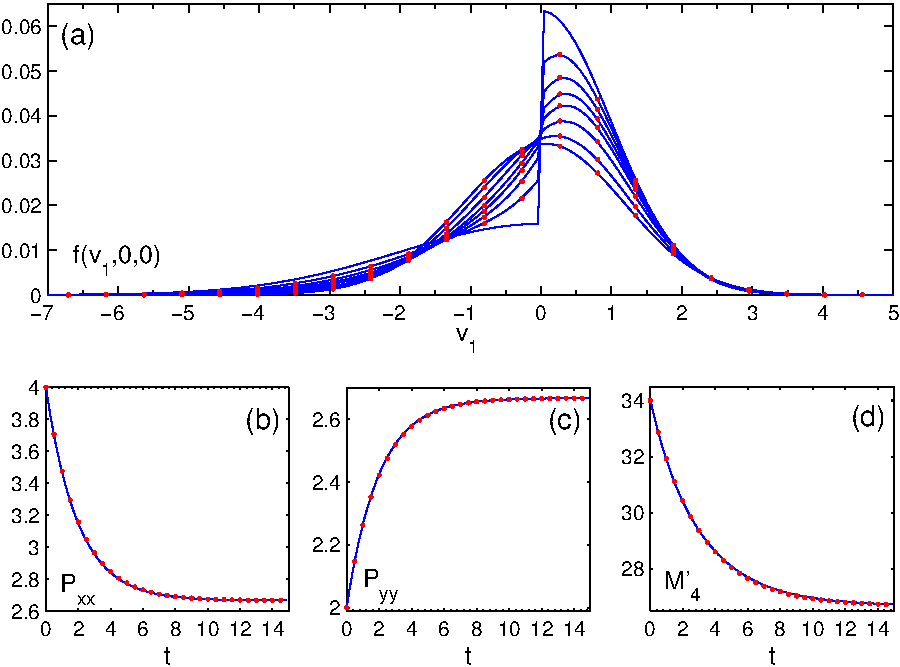
\includegraphics[width=9cm]{Chapter4/IMG/test3_2.pdf}\\
\vskip 0.3cm 
\centering 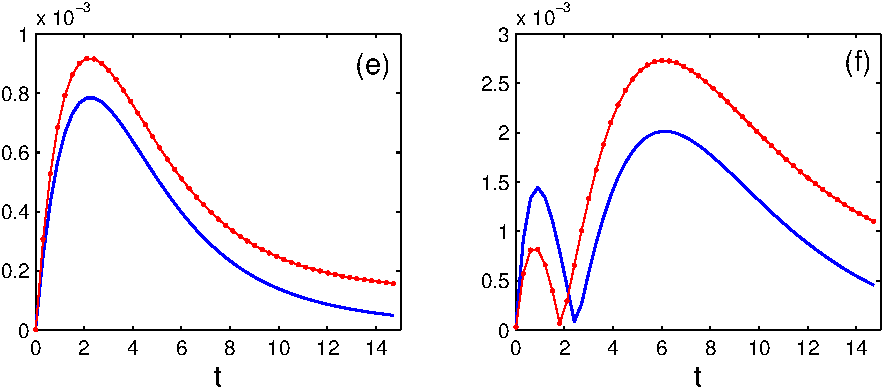
\includegraphics[width=9cm]{Chapter4/IMG/test_error3.pdf}
\caption{ 
	(a) Evolution of the VDF when the initial VDF at $v_1=+0$ is four times larger than at $v_1=-0$. From top to bottom (at $v_1>0$), the times corresponding to the lines are $t=0, 0.5, 1, 1.5, 2, 3, 5$, and $9$, respectively. (b-d) Evolution of the second- and fourth-order moments. Relative error (e) $|p^{nu}_{xx}-p_{xx}|/p_{xx}$ and (f) $|M^{'nu}_{4}-M_{4}^{'}|/M_{4}^{'}$ when $N=42$. Dots are the numerical results when $N_1=N_2=N_3=42$, solid lines in (a), (e), and (f) are the numerical results with $N_1=256, N_2,N_3=42$, while solid lines in (b-d) are analytical solutions. Other parameters are $L_v=11$, $R=2\sqrt{2}L_v/(3+\sqrt{2})$, and $M=5$ with Eq.~\eqref{kernel_FSM_mode}.
} 
\label{test3}
\end{figure}


\subsection{Discontinuous velocity distribution function}

The initial VDF used in the preceding case is smooth, where the spectral accuracy of FSM can be proven analytically~\cite{Mouhot2006}. Now we consider the case where the initial VDF is not smooth, but has an abrupt jump at $v_1=0$:
\begin{equation}\label{initial_3}
f(\bm{v},t=0)=\frac{1}{3(2\pi)^{3/2}}
\begin{cases}
4\exp\left(-\frac{{v^2}}{2}\right) , & v_1\ge0,  \\
\exp\left(-\frac{v_1^2}{8}-\frac{v_2^2+v_3^2}{2}\right), &  v_1<0.
\end{cases}
\end{equation}

Although the analytical solution for the VDF cannot be obtained, it can be shown analytically that the evolution of the second- and fourth-order moments is given by
\begin{equation}\label{initial_33}
\begin{aligned}[b]
  P_{xx} = \frac{4}{3}\exp\left(-\frac{t}{2}\right)+\frac{8}{3}, \\
  P_{yy} = -\frac{2}{3}\exp\left(-\frac{t}{2}\right)+\frac{8}{3}, \\
  M'_{4} = \int fv^4d\bm{v}=\frac{22}{3}\exp\left(-\frac{t}{3}\right)+\frac{80}{3}.
 \end{aligned}
\end{equation}


Figure~\ref{test3} demonstrates that the FSM can accurately capture the evolution of second- and fourth-order moments, even when the initial VDF has a large jump at $v_1=0$. Also, no Gibbs oscillation has been observed in the central region of VDF where the abrupt jump exists; only in the tails do we find small Gibbs oscillations. This is because the convolution in the Boltzmann collision operator can smear out discontinuities.


\begin{figure}[t]
	\centering
	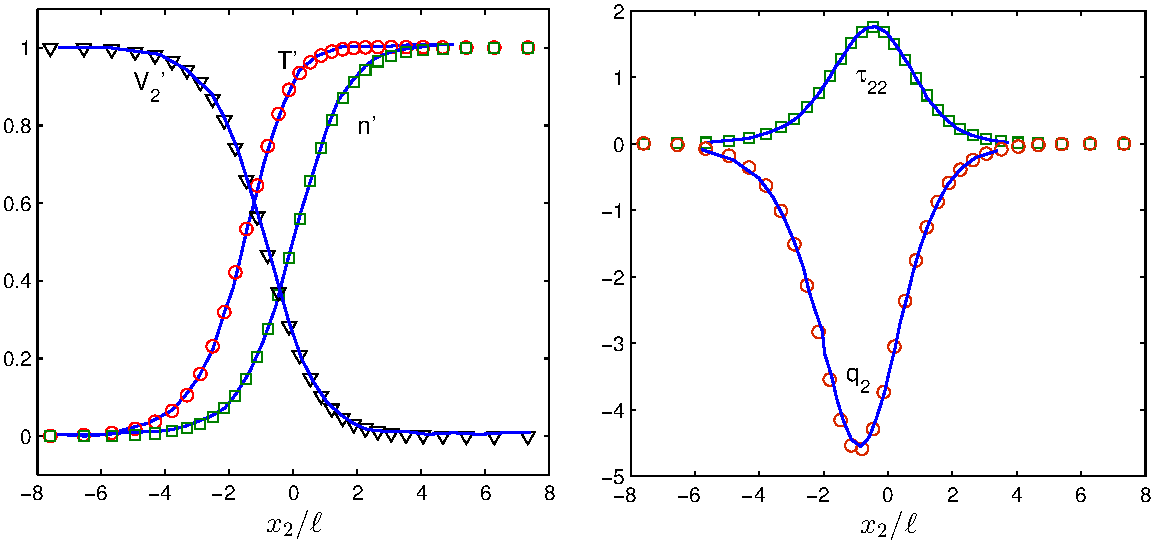
\includegraphics[scale=0.7]{Chapter4/IMG/shock_hard_M3.pdf}
	\caption{
		The structure of normal shock wave when $\text{Ma}=3$, where the reduced macroscopic quantity $\mathcal{M}=\rho, u, T$ is normalized as ${(\mathcal{M}-\mathcal{M}_u)/(\mathcal{M}_d-\mathcal{M}_u)}$, with the subscripts ${u}$ and ${d}$ represent upstream and downstream, respectively. Solid lines are the results from Ref.~\cite{Ohwada1993}, while symbols are our FSM results. 
	}
	\label{shock_Ohwada}
\end{figure}

\section{Accuracy in inhomogeneous problems}\label{CIS_first_time}


The Boltzmann equation is solved by the CIS~\eqref{iteration2}, where the spatial derivative ${\partial {f}}/{\partial\bm{x}}$ is approximated by the second-order upwind scheme.

\index{finite-difference}
\index{upwind}

%In the following calculations, it is found that the use of $M=5$ generates satisfactory results. We use the trapezoidal rule to approximate the kernel mode~\eqref{kernel_mode2}, since for $M=5$ it has almost the same accuracy as that of Gauss-Legendre quadrature but with about 25\% decrease in computational time.

\subsection{Normal shock waves}
\index{shock wave}

\begin{figure}[t]
	\centering
	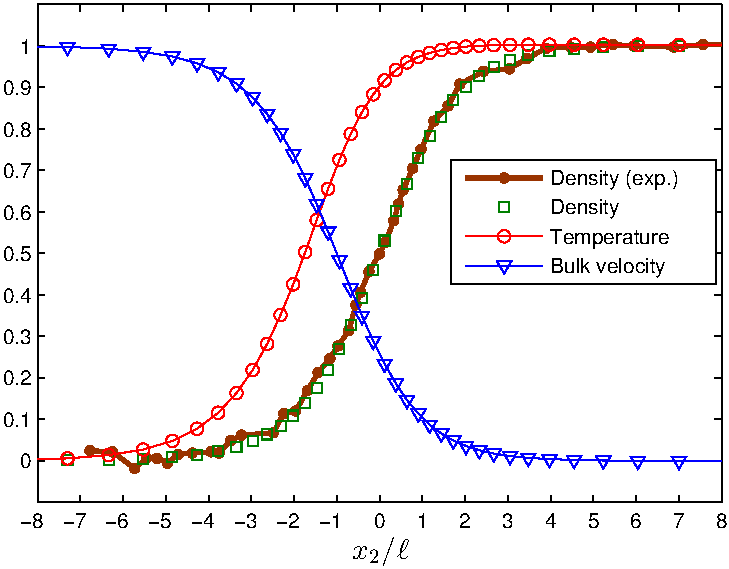
\includegraphics[width=7cm]{Chapter4/IMG/shock_exp.pdf}
	\caption{
		Reduced number density, temperature, and bulk velocity for the normal shock wave of $\text{Ma}=2.80$ in the argon gas, with the upstream temperature of $298\pm3$~K. The experimental density is obtained from Ref.~\cite{Kowalczyk2008}. Numerical parameters are the same as those in Fig.~\ref{shock_Ohwada}.
	}
	\label{shock_exp}
\end{figure}

The normal shock wave problem is ideal for testing the accuracy of FSM in capturing strong rarefaction effects, since this is a one-dimensional problem where the boundary effects are absent. The structure of the planar shock wave varies in the $x_2$ direction. The flow is uniform at the upstream ($x_2=-\infty$) and downstream ($x_2=\infty$) ends. The upstream molecule number density, temperature, and Mach number are denoted by $n_0$, $T_0$, and $\text{Ma}$, respectively, while those of the downstream end is determined through the Rankine-Hugoniot relations: \index{Rankine-Hugoniot relations}
\begin{equation*}%\label{rankine}
\begin{aligned}[b]
n_d=\frac{4\text{Ma}^2}{\text{Ma}^2+3}, \quad
u_d=\sqrt{\frac{5}{96}}\frac{\text{Ma}^2+3}{\text{Ma}},\quad
T_d=\frac{(5\text{Ma}^2-1)(\text{Ma}^2+3)}{16\text{Ma}^2},
\end{aligned}
\end{equation*}
hence the normalized VDF at the upstream end is
\begin{equation}\label{shock_upstream}
    {f}=\frac{1}{{\pi}^{3/2}}\exp\left[-{v}_1^2-
    \left({v}_2-\sqrt{\frac{5}{6}}\text{Ma}\right)^2-{v}_3^2\right],
\end{equation}
and that at the downstream end is
\begin{equation}\label{down_upstream}
    {f}=\frac{n_d}{(\pi{T_d})^{3/2}}\exp\left[-\frac{{v}_1^2+
    ({v}_2-u_d)^2+{v}_3^2}{T_d}\right].
\end{equation}


\subsubsection{Hard-sphere potential}
\index{numerical kernel method}

We first consider the shock wave in a gas of HS molecules. Ohwada solved the Boltzmann equation by means of the numerical kernel method~\cite{Ohwada1993}. For comparison, 
we set $L$ to be the mean free path in the upstream part
\begin{equation}
\lambda_0=\frac{16}{5\pi}\sqrt{\frac{\pi}{2mk_BT_0}}
\frac{\mu}{n_0},
\end{equation} 
and $\text{Kn}=5\pi/16$. Figure~\ref{shock_Ohwada} shows the shock wave structure for a Mach number of 3. In FSM the velocity domain $[-10,10]^3$ is uniformly divided into $42\times42\times42$ grid points, and $M=5$. It can be seen that the two deterministic numerical methods for the Boltzmann equation give identical results.


\begin{figure}[t]
	\centering
	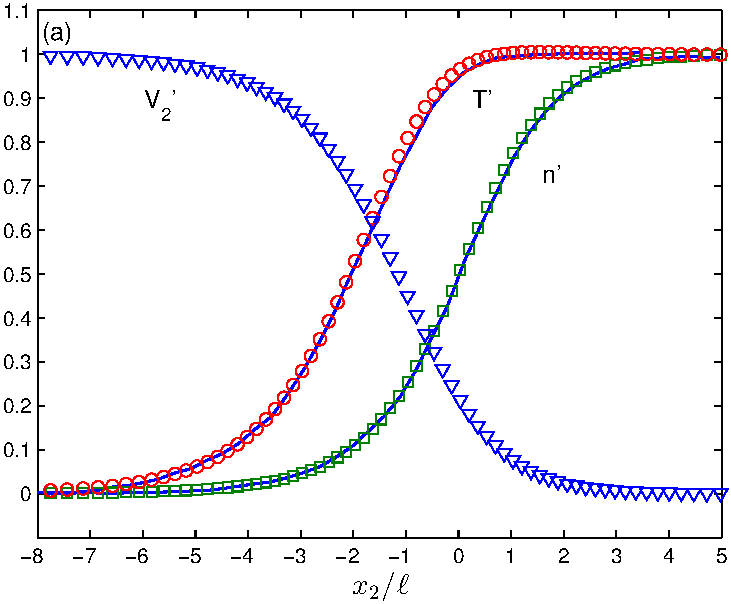
\includegraphics[width=6cm]{Chapter4/IMG/shock_M5_compare2.pdf} \hskip 0.5cm
	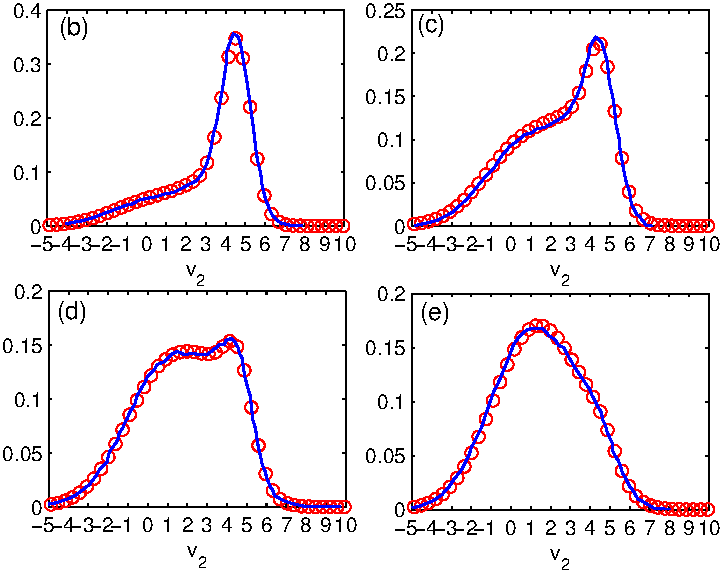
\includegraphics[width=6.2cm]{Chapter4/IMG/shock_LJ_M5_dist.pdf}
	\caption{
		(a) Reduced molecular number density, temperature, and bulk velocity for the normal shock with $\text{Ma}=5$ in argon gas (Lennard-Jones potential). \index{velocity distribution function!marginal}The marginal VDF $\int\int fdv_1dv_3/n$ vs $v_2$ is presented when the reduced density is (b) $0.151$, (c) $0.350$, (d) $0.511$, and (e) $0.759$. Solid lines are the results from Ref.~\cite{Valentini2009}, while symbols are our results from the FSM. The velocity domain $[-18,18]^3$ is divided into $42\times84\times42$ grid points. }
	\label{shock_MD}
\end{figure}



\subsubsection{Lennard-Jones potential}

We then consider argon with the Lennard-Jones \index{Lennard-Jones potential} potential. To compare with experimental data~\cite{Kowalczyk2008}, we set the upstream temperature to be $T_0$ = 298 K, $L$ to be the mean free path in the upstream part,
and hence $\text{Kn}=5\pi/16$ in Eq.~\eqref{LJ_kernel}. Good agreement between the numerical and experimental density profiles is seen in Fig.~\ref{shock_exp}. The agreement is due to the fact that we have correctly incorporated the shear viscosity of argon into the collision kernel, shown in Eq.~\eqref{kernel_spectral}. 


\index{molecular dynamics simulation}
Finally, we solve the Boltzmann equation for argon with the Lennard-Jones potential~\eqref{Lennard_Jones_chapter} and compare our results with molecular dynamics simulation~\cite{Valentini2009}. For comparison, we set the upstream temperature to be $T_0$ = 300 K, $L$ to be the mean free path in the upstream part and $\text{Kn}=5\pi/16$. Fig.~\ref{shock_MD} shows the shock wave structure for Mach number of 5, as well as the marginal VDFs. The FSM produces nearly the same results as the molecular dynamics simulation, not only in macroscopic quantities, but also in mesoscopic VDFs. Note that in this case the downstream temperature is about 2600~K. The excellent agreement with molecular dynamics data illustrates that the collision kernel~\eqref{LJ_kernel} for the Lennard-Jones potential works well in this temperature range.


\subsection{Force-driven Poiseuille flows}\label{force_driven}
%\index{Fourier flow}
%\index{Couette flow}
\index{Poiseuille flow}


Consider a rarefied monatomic gas between two parallel infinite plates located at $x_2=L/2$ and $x_2=-L/2$. The walls are stationary, and the temperature is kept at $T_0$. The gas is subject to a uniform external acceleration $a_1$ in the $x_1$ direction; the acceleration term $\bm{a}\cdot\partial f/\partial \bm{v}$ is calculated according to the Fourier transform derivative theorem. Diffuse boundary condition is employed to account for the wall effects.


\begin{figure}[t]
	\centering
	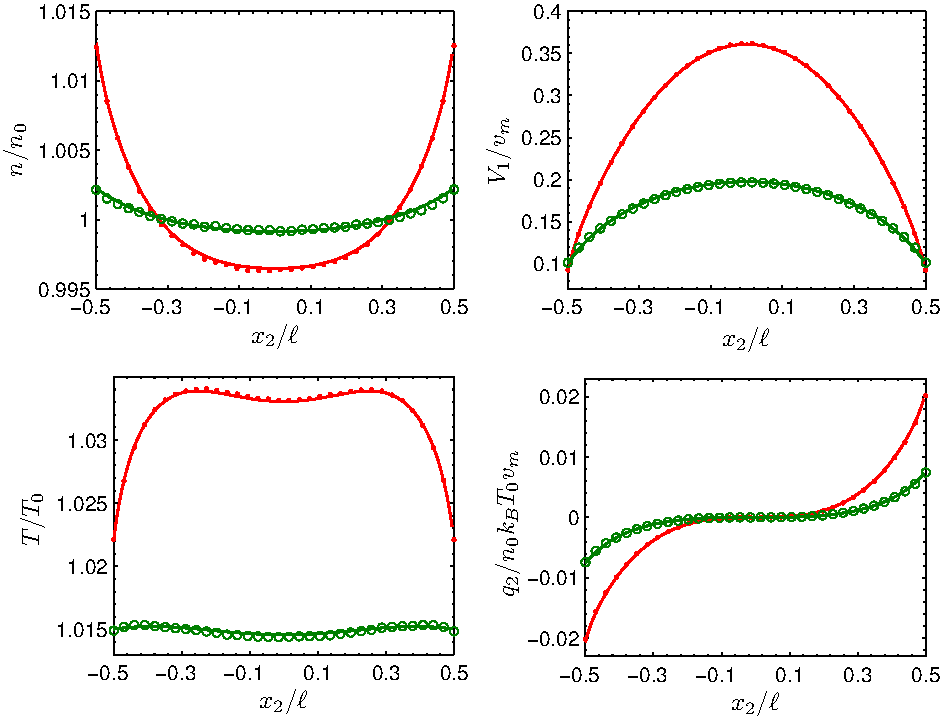
\includegraphics[width=12cm]{Chapter4/IMG/poiseuille_hard.pdf}
	\caption{
		The density, velocity, temperature, and heat flux in the force-driven Poiseuille flow of HS molecules when $\text{Kn}=0.1$ (dots) and $\text{Kn}=0.5$ (open circles). Solid lines are FSM results, while symbols are DSMC results~\cite{Meng2013JCP}.
	}
	\label{poiseuille_fig}
\end{figure}



We solve the discretized Boltzmann equation by the CIS. At the $(k+1)$-th iteration step, the VDF at the wall (entering the cavity) is determined according to the diffuse boundary condition, using the VDF at the same position at the previous iteration step:
\begin{equation}\label{wall_boundary}
\begin{aligned}[b]
{f}^{(k+1)}=&\frac{{n}}{{\pi}^{3/2}}\exp[-({v}_1+{u}_w)^2-{v}_2^2-{v}_3^2],
\ \ \ \operatorname{for} \ {v}_2\le0, \\
{n}=&2\sqrt{\pi}\int_{{v}_2<0}
{v}_2
{f}^{(k)}({x}_2=-0.5,{v})d\bm{v},
\end{aligned}
\end{equation}
This numerical scheme is efficient when the Knudsen number is not small. However, the total mass is not conserved since the mass flux entering the computational domain at the $(k+1)$-th step (which is equal to that leaving the computational domain at the $k$-th step) is not equal to that leaving the computational domain at the $(k+1)$-th step. To overcome this, at the end of each iteration, the VDF is re-scaled so that the total mass is conserved~\cite{Mieussens2004}. Physically, when the average molecular number density $n_0$ and the intermolecular potential are known, the stationary state will be uniquely determined. 



%
%\begin{figure}[t]
%	\centering
%	\includegraphics[width=5.5cm]{lid_arg_Knvhs01u.pdf}
%	\quad
%	\includegraphics[width=5.5cm]{lid_arg_Knvhs01q.pdf}\\
%	\vskip 0.2cm
%	\includegraphics[width=5.5cm]{lid_arg_Knvhs1u.pdf}
%	\quad
%	\includegraphics[width=5.5cm]{lid_arg_Knvhs1q.pdf}
%	\\
%	\vskip 0.2cm
%	\includegraphics[width=5.5cm]{lid_arg_Knvhs10u.pdf}
%	\quad
%	\includegraphics[width=5.5cm]{lid_arg_Knvhs10q.pdf}
%	\caption{Temperature contours and streamlines (velocity: first column; heat flux: second column) in the lid-driven cavity flow of argon gas. From top to bottom, the Knudsen number $\text{Kn}_{vhs}$ defined in Eq.~\eqref{Kn_VHS} in each column is 0.1, 1 and 10, respectively.  Here and after, the abscissa represents the $x_1$-axis, while the ordinate represents the $x_2$-axis.  } 
%	\label{lid}
%\end{figure}

Consider HS molecules when $\text{Kn}=0.1$ and $0.5$. The normalized acceleration is $0.11$ and the wall temperature is $T_0$=273~K. The spatial region (halved due to the symmetry) is divided into $50$ unequally spaced cells with more cells near the boundary. The maximum velocity is at $L_v=6$, and there are 32 velocity mesh points in each direction. The numerical results are depicted in Fig.~\ref{poiseuille_fig}, where good agreements can be found. Note that in this case, the temperature profile has double peaks, which is in sharp contrast with the parabolic profiles predicted by the NSF equations~\cite{Zheng2002}. 

%
%\subsection{Lid-driven cavity flow}
%
%
%
%
%The lid-driven cavity flow is a canonical problem in rarefied gas flows, since it clearly shows the non-equilibrium phenomena where the heat flux is from low-temperature region to high-temperature region, see Fig.~\ref{lid}. The DSMC is extremely time-consuming (i.e., takes about 1000 hours) to find the steady-state solution due to the low velocity near the bottom plate~\citep{John2010,John2011}. Even when the velocity of the moving upper lid is so small that the linearized Boltzmann equation can be applied, the low-noise DSMC method~\citep{Radtke2011} takes more than 1 day to achieve reasonably resolved results when the Knudsen number based on the MFP of variable HS model is $\text{Kn}_{vhs}=0.1$. 
%
%%\begin{figure}[t]
%%	\centering
%%	\includegraphics[scale=0.4]{lid_central_horizontal.pdf}
%%	\includegraphics[scale=0.4]{lid_central_vertical.pdf}\\
%%	\includegraphics[scale=0.4]{lidT.pdf}
%%	\caption{
%%		(Top) Comparisons of the velocity and heat flux profiles between argon and HS gases in the lid-driven cavity flow. (Left) At $x_2=0.5$ and (right) At $x_1=0.5$. Solid (or dashed) lines are the results for argon with $\text{Kn}_{vhs}=0.1$ (or 10), while  circles (or stars) are the results for the HS gas with $\text{Kn}_{vhs}=0.132$ (or 13.2). (Bottom) Comparisons of temperature profiles between argon and HS gases in the lid-driven cavity flow. Filled (open) markers: $x_1=0.5$ $(x_2=0.5)$. 
%%	} 
%%	\label{lidvqt}
%%\end{figure}
%
%We solve this problem (for argon gas, the upper lid velocity of 50~m/s, and a wall temperature of 273~K) in a $51\times51$ nonuniform spatial grid (with most of the grid points located in the vicinity of walls): 
%\begin{equation}\label{spatial_d}
%x=(10-15s+6s^2)s^3, 
%\end{equation}
%with $s=(0,1,\cdots,N_s)/N_s$. The minimum length of the spatial cell is $7.8\times10^{-5}$, while the maximum is 0.0375. For $\text{Kn}_{vhs}=0.1$ and 1,  $32\times32\times12$ grid points in velocity space are used, while for $\text{Kn}_{vhs}=10$, there are $64\times64\times12$ velocity grid points, with most of the grid points located in $v_1,v_2\sim0$ to capture the discontinuities in VDF, see Eq.~\eqref{nonuniform_v}. The number of uniform frequency components is $32\times32\times24$. The Boltzmann collision operator is approximated by the FSM with $M=6$. 
%
%%\begin{equation}
%%||\epsilon||_2=max\left\{\sqrt{\frac{\int|u_1^{k+1}-u_1^k|^2dx_1dx_2}{\int|u_1^k|^2dx_1dx_2}},\sqrt{\frac{\int|u_2^{k+1}-u_2^k|^2dx_1dx_2}{\int|u_2^k|^2dx_1dx_2}}\right\},
%%\end{equation} 
%
%The convergence rate of our iterative scheme is proportional to the Knudsen number. For $\text{Kn}_{vhs}=0.1$ and 1, starting from the global equilibrium state, the FSM takes 110 and 14 minutes, respectively, to produce a converged solution,  when the relative error in flow velocity between two consecutive iteration steps, is less than $10^{-5}$.
%
%Fig.~\ref{lid} shows the calculated temperature contours and streamlines in the lid-driven cavity flow of argon gas with diffuse boundary conditions. Compared to DSMC, these solutions are free of noise. We have also simulated the flow of a HS gas, with the same values of the normalized wall velocity and shear viscosity (the Knudsen number $\text{Kn}$ are the same, but $\text{Kn}_{vhs}$ are different). Comparisons of the velocity, temperature, and heat flux  between the two inverse power-law molecular models demonstrate that the molecular model (reflected in terms of the collision kernel) has little influence on the flow pattern in this case, see Ref.~\cite{lei_Jfm}.




\subsection{Thermal transpiration}\label{chapter_FSM_tc}

\begin{figure}[p]
	\centering
	{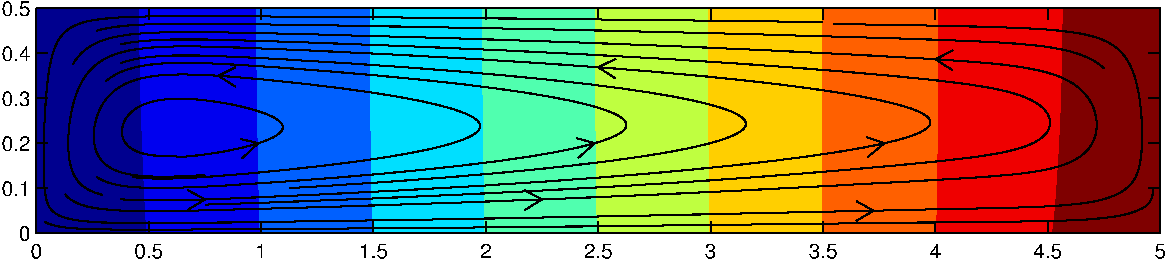
\includegraphics[width=11cm]{Chapter4/IMG/Tc008.pdf}}\\
	{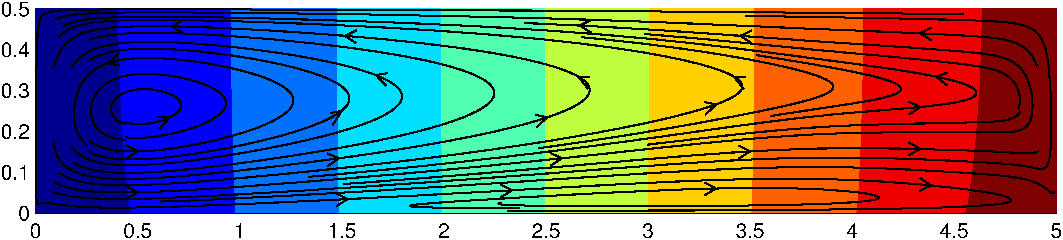
\includegraphics[width=11cm]{Chapter4/IMG/Tc02.pdf}}\\
	{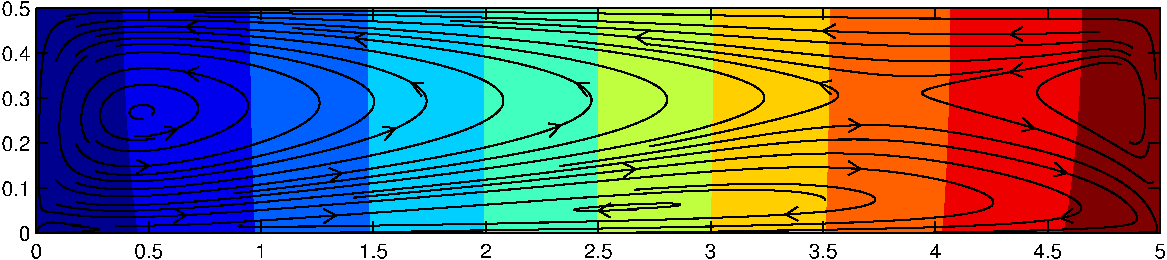
\includegraphics[width=11cm]{Chapter4/IMG/Tc025.pdf}}\\
	{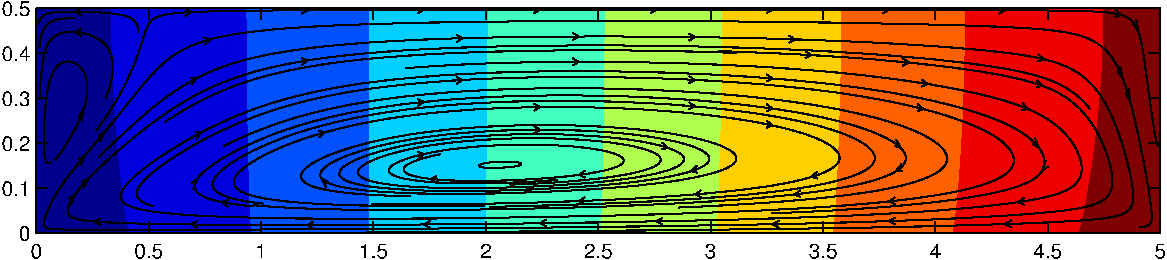
\includegraphics[width=11cm]{Chapter4/IMG/Tc06.pdf}}\\
	{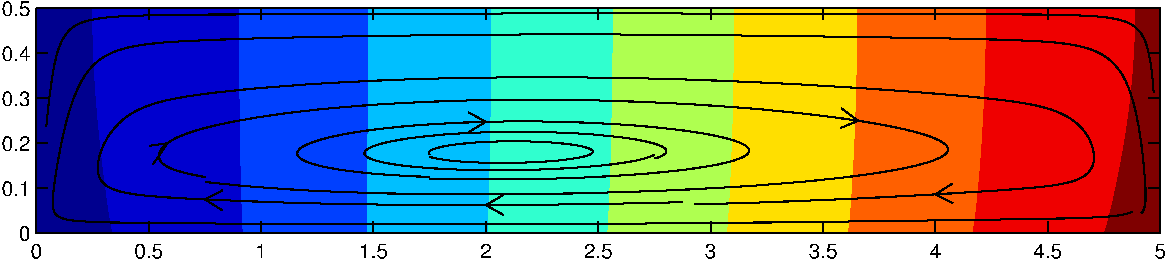
\includegraphics[width=11cm]{Chapter4/IMG/Tc2.pdf}}\\
	{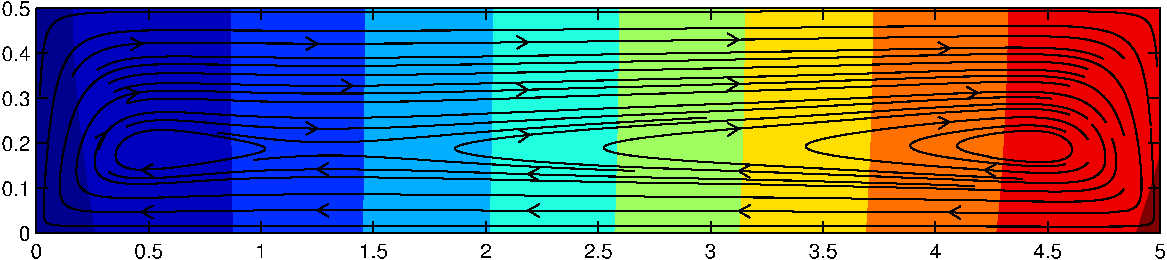
\includegraphics[width=11cm]{Chapter4/IMG/Tc10.pdf}}
	\caption{Temperature contours and velocity streamlines in the thermal transpiration of argon gas within a closed rectangular channel (only the down half domain is shown). In each figure, from left to right, the dimensionless temperature of each contour is $1+0.1i$, where $i=1,2,\cdots,9$. From the top to bottom, $\text{Kn}=0.08$, 0.2, 0.25, 0.6, 2, and 10, respectively. } 
	\label{thermal_creep_channel}
\end{figure}


Consider the thermal transpiration in a 2D closed rectangular channel with a length-to-width ratio of 5. The temperature at the right side is set to be twice that of the left side, while the temperature of the top and bottom walls varies linearly along the channel. Using the mean density, the temperature of the left wall, and the channel width, the Knudsen number is set to be $\text{Kn}=0.08$, 0.2, 0.25, 0.6, 2, and 10. 

Figure~\ref{thermal_creep_channel} presents the  streamlines and temperature distributions inside the channel for the flow of argon gas. Due to symmetry, only half of the spatial domain is shown. At $\text{Kn}=0.08$, the gas flows from the cold region to the hot region along the bottom wall, and returns in the central region. At $\text{Kn}=0.2$, the flow still moves from hot to cold in the central region, however, near the lower wall the flow moves towards the hot region when $x_1<2$ and towards the cold region for at $x_1>2$, i.e., a circulation emerges near the lower corner of the domain. At $\text{Kn}=0.25$, the circulation near the lower wall grows, which divides the flow in the central region into two circulation zones. The lower circulation zone keeps expanding, and pushes the other two circulations in the central region towards the left and right boundaries, as $\text{Kn}$ increases. At $\text{Kn}=0.6$, the flow direction is reversed (as compared to that when $\text{Kn}=0.08$) and only one circulation zone remains near the left wall. The reversal of flow direction persists but the circulations near the left wall gradually disappear as the Knudsen number increases further, for instance, to $\text{Kn}=2$. By $\text{Kn}=10$, the gas near the bottom wall moves from hot to cold, and two clockwise circulations emerge near the left and right sides. Finally, when the flow enters the free molecular regime, the streamline pattern does not change, but the velocity magnitudes are proportional to $1/\text{Kn}$. The magnitudes of density, pressure, and temperature, however, remain unchanged irrespective of the Knudsen number~\cite{lei_Jfm}.

%\begin{figure}
%	\centering
%	{\includegraphics[width=6cm]{tc_free.pdf}}
%	\hskip 0.8cm
%	{\includegraphics[width=5.4cm]{scale_velocity.pdf}}
%	\caption{(Left) The average horizontal velocity varying with $\text{Kn}$ in thermal transpiration inside the closed rectangular channel, in the free molecular regime. In this double logarithmic diagram, the three lines have a slope of 1, demonstrating that the velocity magnitude is proportional to $1/Kn$. (Right) Examples of the linear scalability of the horizontal velocity at $x_1=1.4825$.  } 
%	\label{tc_free}
%\end{figure}

Comparison of the velocity profiles for different molecular models at the start and the end of the transition flow regime  are shown in Fig.~\ref{thermal_creep_v}; it can be seen that the molecular model (reflected in terms of the viscosity index) affects the velocity magnitudes significantly. 

\begin{figure}[t]
	\centering
	{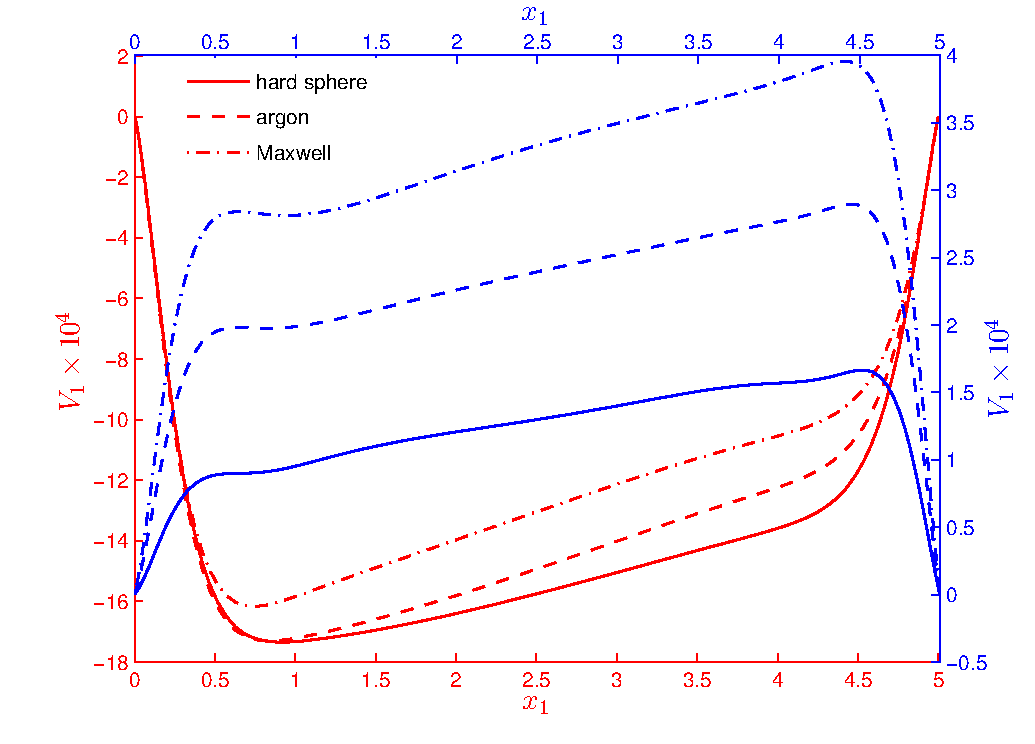
\includegraphics[width=6.5cm]{Chapter4/IMG/tch.pdf}}\hskip 0.4cm
	{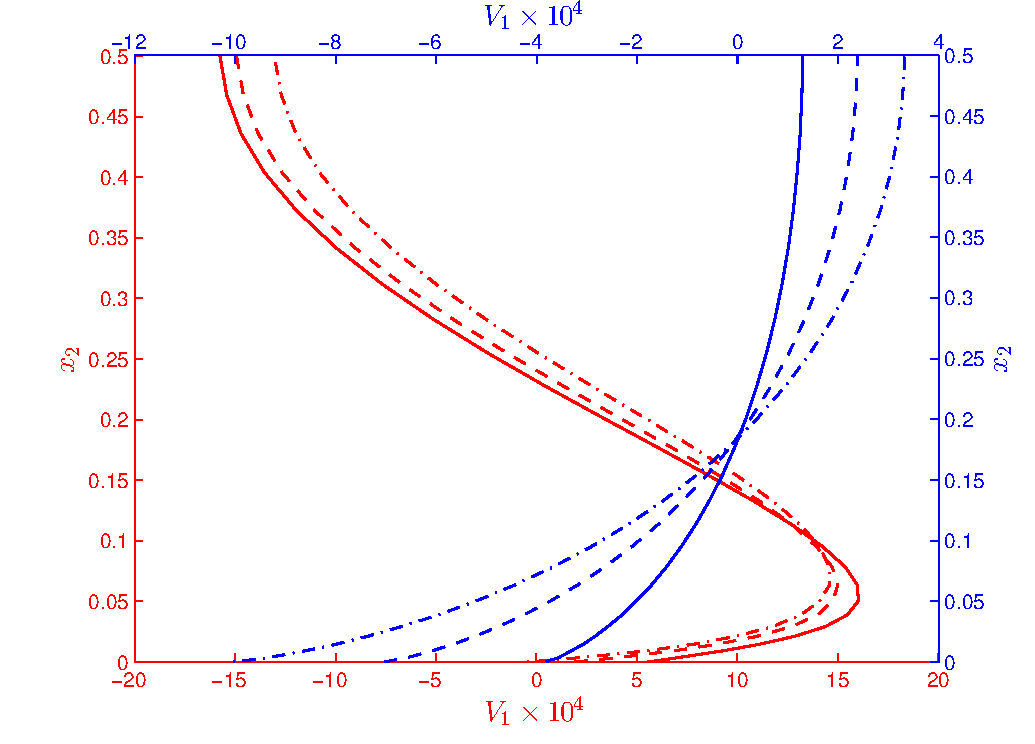
\includegraphics[width=6.5cm]{Chapter4/IMG/tcv.pdf}}
	\caption{Velocity profiles for thermal transpiration within a closed rectangular channel: (a) along the central horizontal line and (b) along the central vertical line. $\text{Kn}=0.08$ and $10$ are represented by the red and blue lines, respectively.} 
	\label{thermal_creep_v}
\end{figure}


%\begin{figure}[t]
%	\centering
%	{\includegraphics[width=8cm]{tc_compare-crop.pdf}}
%	\caption{Net velocity profiles obtained by linear superposition of the velocity profiles of Poiseuille and thermal transpirations between parallel plates, which result in zero mass flow rate. The walls are at $x_2=0$ and $x_2=1$ and the working gas is argon, where the inverse power-law model with $\omega=0.81$ is used.} 
%	\label{tc_mechanism}
%\end{figure}

%The flow patterns shown in Fig.~\ref{thermal_creep_channel} can be understood qualitatively as follows. Starting from the global equilibrium state, the temperature gradient drives the gas molecules to move from cold to hot (thermal transpiration). This process increases the pressure at the right side of the channel while decreasing the pressure at the left. Then, the pressure gradient causes the gas molecules to move to the left (Poiseuille flow). The steady state is reached when the effects of Poiseuille and thermal transpirations cancel each other out, that is, when the net mass flow rate across the lines perpendicular to the top and bottom walls is zero. The horizontal velocity profile can be analysed by assuming the wall temperature gradient to be small (i.e. the channel is long enough) so that the Boltzmann equation can be linearized. In this case, we can directly use the velocity profiles obtained in Sec.~\ref{pt}. Fig.~\ref{tc_mechanism} plots the net velocity profiles in the linear superposition of Poiseuille and thermal transpirations between parallel plates where the net mass flow rate is zero.  The flow velocities are normalised; in real problems, the horizontal velocity is given by (see the first paragraph in Sec.~\ref{tc_linear}):
%\begin{equation}\label{superposition}
%u_1=\beta_T\left\{u_1[h_T]-\frac{\mathcal{M}[h_T]}{\mathcal{M}[h_P]}u_1[h_P]\right\},
%\end{equation}
%where $\beta_T$ is the temperature gradient; in this case, it is about $1/5$.
%
%Now the horizontal velocity profiles in Fig.~\ref{tc_mechanism} can be used to explain the flow patterns in Fig.~\ref{thermal_creep_channel}. 
%From Fig.~\ref{tc_mechanism} we find that, when $\text{Kn}=\sqrt{\pi}/20$, the net horizontal velocity is positive when $x_2<0.25$ and negative otherwise, which agrees well with the flow pattern in Fig.~\ref{thermal_creep_channel}(a). Also, from Fig.~\ref{thermal_creep_v}(a) we find that, at $\text{Kn}=0.08$, $u_1(x_2=0.5)\simeq-0.0018$ near the left side of the channel, which is well predicted by equation~\eqref{superposition} when we choose $\text{Kn}=\sqrt{\pi}/20$ and $x_2=0.5$: $u_1(x_2=0.5)\simeq(-0.009)/5=-0.0018$. Furthermore, as $\text{Kn}$ increases, the magnitude of the horizontal velocity at $x_2=0.5$ decreases (Fig.~\ref{tc_mechanism}). This is in accordance with the horizontal velocity profiles shown in Fig.~\ref{thermal_creep_v}(a), where the velocity magnitude decreases as $x_1$ increases from 1 to 4, because the local Knudsen number increases along the channel as a result of increasing temperature  and decreasing particle number density.  When $\text{Kn}=\sqrt{\pi}/10$ (and $\sqrt{\pi}/8$), the net horizontal velocity in Figure~\ref{tc_mechanism} is positive when $0.26>x_2>0.009$ (and $0.28>x_2>0.023$) and negative otherwise. This explains the flow patterns at the right side of the channel, as shown in Figure~\ref{thermal_creep_channel}(b). As $\text{Kn}$ increases, the extent of the region near the bottom wall where the velocity is negative increases (Figure~\ref{tc_mechanism}), so that the circulation near the bottom wall in Figure~\ref{thermal_creep_channel}(c) is larger than that in Figure~\ref{thermal_creep_channel}(b). When $\text{Kn}$ increases above a critical value of around $\sqrt{\pi}/5$, the horizontal velocity in Figure~\ref{tc_mechanism} is negative when $x_2$ is smaller than some fixed value $x_{2c}$ and positive otherwise. In this case, the flow direction is completely reversed in comparison with that at small Knudsen numbers.  When $\text{Kn}>\sqrt{\pi}/2$,  the fixed value is $x_{2c}=0.2$. In Figure~\ref{thermal_creep_channel}(d-f), we see that the gas moves from left to right if $x_2<0.2$, and moves right to left if $x_2>0.2$. 

%\begin{figure}[t]
%	\centering
%	{\includegraphics[width=10cm]{flow_pattern.pdf}}
%	\caption{Thermal transpiration patterns of the argon gas (inverse power-law model with $\omega=0.81$) in the free molecular regime at different values of length-to-height ratio $A$. (a) $A=0.25$, (b) $A=0.5$, (c) $A=1$, and (d) $A=2$. } 
%	\label{flow_pattern}
%\end{figure}

%Note that the above analysis is valid at positions far from the left and right walls; near the ends of the channel, the horizontal velocity is nearly zero and the above analysis fails. This end effect becomes dominant in the whole channel when the molecular mean free path is of the order of half the distance between the left and right walls. When the mean free path is much larger than the wall distance, from figures~\ref{thermal_creep_channel} and~\ref{tc_free} we find that the streamline pattern does not change very much, but the velocity magnitude is inversely proportional to the Knudsen number. In other words, at large Knudsen numbers, the flow pattern is determined by the velocity profiles in Figure~\ref{tc_mechanism} at a critical Knudsen number. In our numerical simulations, we find that the critical Knudsen number varies linearly with the length-to-height ratio $A$ of the channel:
%\begin{equation}
%Kn_c\simeq0.35A.
%\end{equation} 
%For instance, when $A=0.25$, the end effect becomes dominant when $\text{Kn}_c\ge0.09$, and the flow pattern at $\text{Kn}\gg{Kn_c}$ is similar to the flow pattern at $\text{Kn}_c$. Figure~\ref{tc_mechanism} shows that at $\text{Kn}=0.09$ the molecules move from left to right near the bottom wall, and return to the left at $x_2=0.5$, which is exactly the case shown in Figure~\ref{flow_pattern}(a). For $A=0.5$, $\text{Kn}_c=0.18\simeq\sqrt{\pi}/10$,  and from Figure~\ref{tc_mechanism} we see the horizontal flow velocity turns from negative to positive and then back to negative as we move from the bottom wall to the central region, which is the same as in Figure~\ref{flow_pattern}(b). The aspect ratio $A=1$ is a critical case, since near $\text{Kn}_c=0.35\simeq\sqrt{\pi}/5$, the horizontal velocity at $x_2=0.5$ could be negative or positive, depending on whether the local Knudsen number is smaller or larger than $\sqrt{\pi}/5$. That is why the  flow pattern shown in Figure~\ref{flow_pattern}(c) is more complicated. For $A=2$, where $\text{Kn}_c=0.7$, the flow pattern is simpler, and the molecules move from the hot to the cold region near the bottom and return from the cold to the hot region near $x_2=0.5$, see Figure~\ref{flow_pattern}(d). For $\text{Kn}<Kn_c$, the horizontal velocity profiles can be analysed using the data in Figure~\ref{tc_mechanism}. 







%\subsubsection{Flow induced by a temperature discontinuity}
%
%\begin{figure}[t]
%	\centering
%	\includegraphics[width=7cm]{discontinuty_maxwell01.pdf}
%	\quad
%	\includegraphics[width=7cm]{discontinuty_maxwell1.pdf}\\
%	\vskip 0.5cm
%	\includegraphics[width=7cm]{discontinuty_maxwell10.pdf}\\
%	\vskip 0.5cm
%	\includegraphics[scale=0.5]{dis_u.pdf}
%	\quad
%	\includegraphics[scale=0.5]{dis_v.pdf}
%	\caption{Temperature contours and velocity streamlines in the flow in a square box of a Maxwell gas driven by a temperature discontinuity at the bottom left corner. (left) $\text{Kn}=0.1$; (right) $\text{Kn}=1$; (middle row) $\text{Kn}=10$. (Bottom)	Comparison of the velocity profiles for different molecular models. (left) velocity along the central horizontal line and (right) velocity along the central vertical line.   } 
%	\label{dist}
%\end{figure}




%Finally, we consider the gas flow inside a square box that is driven by a temperature discontinuity: the temperature of the left wall is one half that of the other three walls. In terms of the mean density, temperature of the left wall, and the wall distance, $\text{Kn}$ is 0.1, 1, and 10 in the cases we investigate. The half spatial region ($0\le{}x_1\le1$, $0\le{x_2}\le0.5$) is simulated, due to symmetry. The nonuniform spatial grids are $101\times100$ for $\text{Kn}=0.1$, and $51\times30$ for $\text{Kn}=1$ and 10. The velocity grids are $48\times48\times12$ for $\text{Kn}=0.1$ and 1, and $64\times64\times12$ for $\text{Kn}=10$. The temperature contours and velocity streamlines for a Maxwell gas in this configuration are shown in Figure~\ref{dist}. At $\text{Kn}=0.1$, four circulation zones arise.  As $\text{Kn}$ increases, the two circulations near the left and the right walls gradually disappear, while the centre of the largest circulation moves towards the right wall. Note that this problem was previously studied using the original DSMC method~\citep{Huang2013}, and comparison shows that our FSM yields much smoother streamlines than the DSMC method at $\text{Kn}=0.1$. 



%The velocity profiles along the central horizontal and vertical lines are depicted in Figure~\ref{dist},  and clearly show the influence of different molecular models. However, interestingly, the molecular model has little effect on the temperature and heat flux profiles (not shown). %{We have also solved this problem using the BGK model, and found that while the BGK model gives almost identical temperature and heat flux profiles, it cannot recover the velocity profiles.} 
%In the free molecular limit, the density, pressure, and temperature profiles reach fixed values independent of the Knudsen number. The streamline pattern also remains unchanged, except that the velocity magnitudes decrease as $1/\text{Kn}$.



\section{Linearization}\label{linearization_FSM}
\index{linearization}

The linearized BCO~\eqref{BCO_lin_chapter1} cannot be solved by FSM, because in general the perturbation function $\phi(-L_v)\neq\phi(L_v)$. However, the product of the equilibrium distribution function and $\phi$ vanishes at large molecular speed. Therefore, the Boltzmann equation is linearized by expressing the VDF as (the normalization in Section~\ref{Normalization_FSM} is used):
\begin{equation}\label{Chapter_lin_VDF}
f(t,\bm{x},\bm{v})=f_{eq}(\bm{v})+\beta{}h(t,\bm{x},\bm{v})
\end{equation}
with the equilibrium distribution function
\begin{equation}\label{equilibrium_Maxwellian_lin}
f_{eq}(\bm{v})=\pi^{-3/2}\exp(-v^{2}),
\end{equation}
where $\beta$ is a small constant related to the dimensionless strength of perturbation (e.g., in the linear Couette flow $\beta$ is the wall velocity divided by the most probable speed), and $\beta{}h$ is the VDF for small perturbation satisfying $|\beta{}h/f_{eq}|\ll1$. The Boltzmann equation~\eqref{Boltzmann} is linearized to
\begin{equation}\label{Chapter1_Boltzmann_lin}
\frac{\partial {h}}{\partial t}+\bm{v}\cdot\frac{\partial{h}}{\partial
	\bm{x}}
-2\bm{a}\cdot\bm{v}f_{eq}=\mathcal{L}(h)\equiv{}\mathcal{L}^+-\nu_{eq}(\bm{v}){h},
\end{equation}
where 
\begin{equation}\label{linearized1}
\mathcal{L}^+(h)=\iint B(\theta,v_r)  [f_{eq}(\bm{v}')h({\bm{v}}'_{\ast})+f_{eq}(\bm{v}'_\ast)h({\bm{v}}')-f_{eq}(\bm{v})h({\bm{v}}_\ast)]d\Omega d{\bm{v}}_\ast
\end{equation}
can be viewed as a gain term of the linearized BCO, while $\nu_{eq}(\bm{v}){h}$ is the loss term, with the equilibrium collision frequency being
\begin{equation}\label{linearized2}
\nu_{eq}(\bm{v})=\iint{}B(\theta,{v}_r)f_{eq}(\bm{v}_{\ast}) d\Omega{d\bm{v}_\ast}.
\end{equation} 



%
%In the present paper, we \lei{mainly} consider the inverse power-law potentials, where the collision kernels are modeled as~\cite{Lei2013,lei_Jfm}
%\begin{equation}\label{collision_kernel}
%B(|{\bm{u}}|,\theta)=\frac{|{\bm{u}}|^{2(1-\omega)}}{K}	{\sin^{\frac{1}{2}-\omega}\left(\frac{\theta}{2}\right)\cos^{\frac{1}{2}-\omega}\left(\frac{\theta}{2}\right)},
%\end{equation}
%with $\omega$ being the viscosity index (i.e. the shear viscosity $\mu$ of the gas is proportional to $T^\omega$) and $K$ some normalization constants~\cite{lei_Jfm}. HS and Maxwell molecules have $\omega=0.5$ and 1, respectively. \lei{We will also consider the Lennard-Jones potentials (the detailed implementation of which by the fast spectral method can be found in Ref.~\cite{Wu:2015yu}) to demonstrate that the GSIS works for the LBE with general intermolecular potentials}.







The macroscopic quantities deviated from their corresponding values in equilibrium state, such as the number density $\varrho$, bulk velocity $\bm{u}$, temperature $T$, stress tensor $\sigma_{ij}$ and heat flux $\bm{q}$ can be calculated as
\begin{equation}\label{MP}
[\varrho,\bm{u},T,\sigma_{ij},\bm{q}]=
\int\left[1,\bm{v},\frac{2}{3}\left(v^2-\frac{3}{2}\right),2v_{\langle i}v_{j\rangle},\bm{v}\left({v^2}-\frac{5}{2}\right)\right]{h}d\bm{v},
\end{equation}
which, on top of the normalization~\eqref{normalization}, are further normalized by the dimensionless constant $\beta$.


The equilibrium collision frequency can be calculated analytically, or approximated by the algorithm in Appendix~\ref{appen_FSM}, if $\hat{f}$ is replaced by the spectrum of  equilibrium distribution function $\hat{f}_{eq}$. This term only needs to be calculated once, since each spatial cell uses the same equilibrium collision frequency. Typical profiles are shown in Fig.~\ref{collision_frequency}.


The gain term is calculated similarly by the method introduced in the previous chapter. Let
\begin{equation}
\phi_{loss}=\sum_{p,q=1}^{M}\omega_p\omega_q\sin\theta_p\phi_{\alpha+\gamma}(\xi_{\bm{m}},\theta_p,\varphi_q)    \psi_{\gamma}(\xi_{\bm{m}},\theta_p,\varphi_q),
\end{equation}
and $\hat{h}$  the spectrum of $h$. If Eq.~\eqref{kernel_mode2} is approximated by Gauss-Legendre quadrature, its $j$-th Fourier mode of the gain term $\mathcal{L}^+$ is 
\begin{equation}\label{detailed_linear}
\begin{aligned}[b]
\widehat{\mathcal{L}}^+_{\bm{j}}\approx &\frac{4}{\text{Kn}'}\sum_{p,q=1}^{M} \sum_{\bm{l}+\bm{m}=\bm{j}}\omega_p\omega_q\sin\theta_p[\hat{f}_{eq}(\bm{l}){\phi_{\alpha+\gamma}(\xi_{\bm{l}},\theta_p,\varphi_q)}]\cdot[\hat{h}_{\bm{m}}{\psi_{\gamma}(\xi_{\bm{m}},\theta_p,\varphi_q)}]\\
+&\frac{4}{\text{Kn}'}\sum_{p,q=1}^{M} \sum_{\bm{l}+\bm{m}=\bm{j}}\omega_p\omega_q\sin\theta_p[\hat{h}_{\bm{l}}{\phi_{\alpha+\gamma}(\xi_{\bm{l}},\theta_p,\varphi_q)}]\cdot[\hat{f}_{eq}(\bm{m}){\psi_{\gamma}(\xi_{\bm{m}},\theta_p,\varphi_q)}]
\\
-&\frac{4}{\text{Kn}'}\sum_{\bm{l}+\bm{m}=\bm{j}}\hat{f}_{eq}(\bm{l})\cdot[\hat{h}_{\bm{m}}{\phi_{loss}}].
\end{aligned}
\end{equation}
The gain term $\mathcal{L}^+$ can be calculated by the second algorithm in Appendix~\ref{appen_FSM}. Since the Fourier transform of  $\hat{f}_{eq}(\bm{l}){\phi_{\alpha+\gamma}(\xi_{\bm{l}},\theta_p,\varphi_q)}$ and $\hat{f}_{eq}(\bm{m}){\psi_{\gamma}(\xi_{\bm{m}},\theta_p,\varphi_q)}$ can be pre-computed and stored, the computational time of the linearized BCO is nearly the same as that of the full BCO. Therefore, it seems that there is no need to consider the Boltzmann equation in linearized form. However, the following three factors indicate that the linearization is necessary and beneficial: 
\begin{itemize}
	\item In LBE the small signal is magnified thus can be better resolved, while in the full Boltzmann equation this signal might be contaminated by numerical error.
	
	\item In oscillatory flows the time derivative can be removed if one are interested in the ``steady-state'' solution, where the flow oscillation has been fully established (see Chapter~\ref{chap:GSIS_oscillatory}); the use of FSM for LBE facilitates the fast convergence to final solution, without running time-explicit numerical solvers. 
	
	\item For inverse power-law potentials, if we choose $\gamma=(1-\alpha)/2$ in the collision kernel~\eqref{kernel_lei}, the linearized gain term $\mathcal{L}^+(h)$ becomes
	\begin{equation}
	\begin{aligned}[b]
	&\frac{4}{\text{Kn}'}\iint{d\bm{y} d\bm{z}}\delta(\bm{y}\cdot{}\bm{z})(|\bm{y}||\bm{z}|)^{-\gamma}\\ &\times[f_{eq}(\bm{v}+\bm{z})h(\bm{v}+\bm{y})+h(\bm{v}+\bm{z})f_{eq}(\bm{v}+\bm{y})
	-h(\bm{v}+\bm{y}+\bm{z})f_{eq}(\bm{v})]
	\end{aligned}
	\end{equation}
	after the Carleman representation. Since the interchange of $\bm{y}$ and $\bm{z}$ does not change the linearized gain term, Eq.~\eqref{detailed_linear} can be simplified to 
	\begin{equation}\label{detailed_linear_half}
	\begin{aligned}[b]
	\widehat{\mathcal{L}}^+_{\bm{j}}\approx &\frac{8}{\text{Kn}'}\sum_{p,q=1}^{M} \sum_{\bm{l}+\bm{m}=\bm{j} }\omega_p\omega_q[\hat{f}_{eq}(\bm{l}){\phi_{\alpha+\gamma}(\xi_{\bm{l}},\theta_p,\varphi_q)}][\hat{h}_{\bm{m}}{\psi_{\gamma}(\xi_{\bm{m}},\theta_p,\varphi_q)}]\sin\theta_p\\
	-&\frac{4}{\text{Kn}'}\sum_{\bm{l}+\bm{m}=\bm{j} }\hat{f}_{eq}(\bm{l})[\hat{h}_{\bm{m}}{\phi_{loss}}]. 
	%\operatorname{or} \\
	%\widehat{\mathcal{L}}^+_{\bm{j}} \approx 
	%&\frac{8}{\text{Kn}'}\sum_{p,q=1}^{M} \sum_{\bm{l}+\bm{m}=\bm{j} }\omega_p\omega_q[\hat{h}_{\bm{l}}{\phi_{\alpha+\gamma}(\xi_{\bm{l}},\theta_p,\varphi_q)}][\hat{f}_{eq}(\bm{m}){\psi_{\gamma}(\xi_{\bm{m}},\theta_p,\varphi_q)}]\sin\theta_p
	%\\
	%-&\frac{4}{\text{Kn}'}\sum_{\bm{l}+\bm{m}=\bm{j}}\hat{f}_{eq}(\bm{l})[\hat{h}_{\bm{m}}{\phi_{loss}}].
	\end{aligned}
	\end{equation}
	Therefore, the computational cost will be reduced by half when compared to that of the full Boltzmann equation. 
	
\end{itemize}


\index{Lennard-Jones potential}
\subsection{Lennard-Jones potential}\label{linear_LJ_FSM}

When the Lennard-Jones potential is considered, after the normalization in Section~\ref{Normalization_FSM}, the collision kernel $B(\theta,v_r)$ in Eqs.~\eqref{linearized1} and~\eqref{linearized2} becomes~\cite{wuPoF2015}:
\begin{equation}\label{LJ_collision_kernel}
B(\theta,v_r)=(n_0d_{LJ}^2L)\sigma_Dv_r,
\end{equation} 
where the differential cross-section, after the Carleman representation, is
\index{differential cross-section}
\begin{equation}
\sigma_D=\sigma_D\left(2\text{arctan}\frac{|y|}{|z|},v_m\sqrt{y^2+z^2}\right)\equiv\sigma_D'(|y|,|z|).
\end{equation}
In general, $y$ and $z$ in $\sigma_D'(|y|,|z|)$ cannot be separated as $\sigma_1(|y|)\sigma_2(|z|)$, and the kernel mode 
$\beta(\bm{l},\bm{m})$ can only be simplified to
\begin{equation}\label{kernel_LJ_mode00}
\begin{aligned}[b]
\beta(\bm{l},\bm{m})=&(n_0d_{LJ}^2L)\iint {}d\bm{e}'d\bm{e} \delta(\bm{e}\cdot{\bm{e}'})\\
\times&
\int_{-R}^R\int_{-R}^R|\rho\rho'|\sigma'_D(|\rho|,|\rho'|)\exp(i\rho\xi_{\bm{l}}\cdot{\bm{e}}+i\rho'\xi_{\bm{m}}\cdot{\bm{e}'})d\rho d\rho'.
\end{aligned}
\end{equation}



To enable the FFT-based convolution, the integration with respect to $\rho$ is approximated by a numerical quadrature~\cite{Hu2012,wuPoF2015}, and the integration with respect to $\rho'$ is calculated accurately, or vise versa. Suppose $\rho_r$ and $\omega_r$ with $r=1,2,\cdots,M_r$ are the abscissas and weights of a quadrature in the region $[0,R]$, Eq.~\eqref{kernel_LJ_mode00} becomes
%\footnote{For the Lennard-Jones potential, for each relative collision energy $E$, the differential cross-section is a continuous function of the deflection angle at $E=u^2k_BT_0/(2\epsilon)=(\rho_r^2+\rho'^2)k_BT_0/(2\epsilon)\lesssim1$ and has one discontinuous point at $E>1$~\cite{Sharipov_trans}. Therefore, the integration region $0\le\rho\le{}R$ is divided into two regions: the first region $[0,\sqrt{2\epsilon/k_BT_0}]$ is divided into 9 uniform sections, while the second region $[\sqrt{2\epsilon/k_BT_0},R]$ is discretized according to the Gauss-Legendre quadrature of order 7. So the number of points in the discretization of  $\rho$ is $M_r=16$.} 
\begin{equation}
\beta(\bm{l},\bm{m})=(n_0d_{LJ}^2L)\sum_{r}\omega_r\iint  \delta(\bm{e}\cdot{\bm{e}'})\phi(\rho_r,\xi_{\bm{l}}\cdot{\bm{e}})\psi(\rho_r,\xi_{\bm{m}}\cdot{\bm{e}'})d\bm{e}'d\bm{e},
\end{equation} 
where $\psi(\rho_r,s)=2\int_0^R \rho'\sigma'_D(\rho_r,\rho')\cos(\rho's) d\rho'$ and $\phi(\rho_r,s)=2\rho_r\cos(\rho_rs)$. Then, following the straightforward algebraic calculation in Section~\ref{fourier_galerkin_spectral}, we have
\begin{equation} \label{kernel_modee}
\beta(\bm{l},\bm{m})= 4(n_0d_{LJ}^2L)\sum_{p,q,r=1}^{M,M,M_r}{\omega_p\omega_q\omega_r}
\phi(\rho_r,\xi_{\bm{l}}\cdot{\bm{e}_{\theta_p,\varphi_q}}) 
\psi'\left(\rho_r,\xi^\perp_{\bm{l}}\
\right) \sin\theta_p,
\end{equation}
where
%\footnote{We first check the continuity of the differential cross-section as $\rho'$ goes from 0 to $R$. If $\sigma'_D(\rho_r,\rho')$ is continuous, then Eq.~\eqref{psi_expression} is approximated by the Gauss-Legendre quadrature of order 120. Otherwise, suppose $\sigma'_D(\rho_r,\rho')$ is discontinuous at $\rho'=\rho'_d$, then the region $\rho'\in[0,\rho'_d)$ is discretized non-uniformly by 60 points, with most of the points located near $\rho'_d$, while the remaining region $\rho'\in[\rho'_d,R]$ is approximated by the Gauss-Legendre quadrature of order 60. In the numerical integration of $\psi'$, a differential cross-section with deflection angle less than 0.05 radians is neglected. Finally, when $\psi'\left(\rho_r,s\right)$ is obtained, $\psi'\left(\rho_r,\xi^\perp_{\bm{l}}\right)$ is calculated through cubic interpolation. } 
\begin{equation}\label{psi_expression}
\psi'(\rho_r,s)=2\pi\int_0^R \rho'\sigma'_D(\rho_r,\rho')J_0(\rho' s)d\rho'.
\end{equation}

%
%\begin{figure}[t]
%	\centering
%	\includegraphics[scale=0.7]{Fourier_nonlinear_LJ}
%	\caption{Density and temperature profiles in the nonlinear Fourier flow between two parallel plates when $\delta_{rp}=0.1$ (top row) and $\delta_{rp}=1$ (bottom row). Dash-dotted lines: a HS gas; Solid lines: He; Dashed lines: Kr.}
%	\label{Fourier_nonlin}
%\end{figure}


Thus, the BCO for the Lennard-Jones potential can be calculated through the FFT-based convolution, with a computational cost of $O(M^2M_rN^3\log{N})$. Normally $M_r\sim N$, so the computational cost for the Lennard-Jones potential is high than the modeled collision kernel~\eqref{kernel_lei} by about one order of magnitude. Detailed numerical method to calculate the differential cross-section and the corresponding kernel mode is given in Ref.~\cite{wuPoF2015}. 


\subsection{Accurate transport coefficients}\label{accurate_transport}
\index{transport coefficient}


Note that the shear viscosity~\eqref{shear_CE_viscosity} is derived based on the eigenvalues and eigenfunctions of the LBE for Maxwell molecules. For general intermolecular potentials, however, Eq.~\eqref{shear_CE_viscosity} is not accurate, and its high-order correction is cumbersome. Here we show how to obtain accurate transport coefficients of the Boltzmann equation via FSM. 

According to the Chapman-Enskog expansion, the exact shear viscosity $\mu$ and thermal conductivity $\kappa$ of the Boltzmann equation are calculated by
\begin{equation}
\begin{aligned}[b]
\mu=\frac{mv_m}{d_{LJ}^2}\int h_\mu(v)v_1v_2dv\equiv\frac{mv_m}{d_{LJ}^2}\mu',\\
\kappa=\frac{k_Bv_m}{d_{LJ}^2}\int h_\kappa(v)v_1\left(v^2-\frac{5}{2}\right)dv\equiv\frac{k_Bv_m}{d_{LJ}^2}\kappa',
\end{aligned}
\end{equation}
where $\mu'$ and $\kappa'$ are the reduced viscosity and thermal conductivity, respectively. The two functions $h_\mu(v)$ and $h_\kappa(v)$ satisfy the following integral equations if we choose $n_0d_{LJ}^2L=1$ in the collision kernel:
\begin{eqnarray}\label{transport}
\begin{aligned}[b]
\mathcal{L}(h_\mu)=-2f_{eq}v_
1v_2,\\
\mathcal{L}(h_\kappa)=-f_{eq}v_1\left(v^2-\frac{5}{2}\right), \ \ \ \text{and} \int h_\kappa v_1dv=0.
\end{aligned}
\end{eqnarray}
To find $h_\mu$, we use the following iterative scheme:
\begin{equation}\label{iteration_thermal}
h_\mu^{(k+1)}=\frac{\mathcal{L}^+(h_\mu^{(k)})+2f_{eq}v_1v_2}{\nu_{eq}},
\end{equation} 
while to find $h_\kappa$, we use
\begin{equation}\label{iteration_thermal2}
\begin{aligned}[b]
\widetilde{h}_\kappa^{(k+1)}=\frac{\mathcal{L}^+(h_\kappa^{(k)})+f_{eq}v_1\left(v^2-\frac{5}{2}\right)}{\nu_{eq}},\\
{h}_\kappa^{(k+1)}=\widetilde{h}_\kappa^{(k+1)}-2f_{eq}v_1{\int \widetilde{h}_\kappa^{(k+1)} v_1 dv}.
\end{aligned}
\end{equation} 
% transport coefficient
\begin{table}[t]
	\caption{Comparisons of reduced transport coefficients obtained from the FSM at temperature 300~K~\cite{wuPoF2015} with those from the variational method with first- and third-order Chapman-Cowling approximation~\cite{variational}.   }
	\centering
	\begin{tabular}{cccccccccccc}
		\hline
		Gas & $\mu'^{[1]}$ & $\mu'^{[3]}$ &   FSM  $\mu'$ & $\kappa'^{[1]}$ & $\kappa'^{[3]}$ &  FSM  $\kappa'$ \\ 
		\hline 
		He & 0.1773 & 0.1787  & 0.1789  & 0.6650 & 0.6732  & 0.6742 \\
		Ne & 0.1477 & 0.1488  & 0.1486  & 0.5539 & 0.5602  & 0.5596 \\
		Ar & 0.1129 & 0.1131  & 0.1132  & 0.4234 & 0.4248  & 0.4251 \\
		Kr & 0.0969 & 0.0969  & 0.0967  & 0.3632 & 0.3635  & 0.3629 \\
		Xe & 0.0892 & 0.0893  & 0.0894  & 0.3348 & 0.3349  & 0.3354 \\
		\hline
	\end{tabular}
	\label{transport_coe} 
\end{table}



%\begin{table}[t]
%	\caption{Comparisons of reduced transport coefficients obtained from the FSM at temperature 300~K~\cite{wuPoF2015} with those from the variational method with first- and third-order Chapman-Cowling approximation~\cite{variational} and the discrete velocity method~\cite{Sharipov_trans}.   }
%	\centering
%	\begin{tabular}{cccccccc}
%		\hline
%		Gas & $\mu'^{[1]}$ & $\mu'^{[3]}$ &    DVM $\mu'$ & FSM  $\mu'$\\ 
%		\hline 
%		He & 0.1773 & 0.1787 & 0.1787 & 0.1789 \\
%		Ne & 0.1477 & 0.1488 & 0.1480 & 0.1486   \\
%		Ar & 0.1129 & 0.1131 & 0.1130 & 0.1132  \\
%		Kr & 0.0969 & 0.09690 & 0.0968 & 0.0967  \\
%		Xe & 0.0892 & 0.0893 & 0.0892 & 0.0894 \\
%		\hline
%		Gas & $\kappa'^{[1]}$ & $\kappa'^{[3]}$ &    DVM $\kappa'$ & FSM  $\kappa'$\\ 
%		He & 0.6650 & 0.6732 & 0.6740 & 0.6742 \\
%		Ne & 0.5539 & 0.5602 & 0.5600 & 0.5596  \\
%		Ar & 0.4234 & 0.4248 & 0.4260 & 0.4251  \\
%		Kr & 0.3632 & 0.3635 & 0.3645 & 0.3629  \\
%		Xe & 0.3348 & 0.3349 & 0.3358 & 0.3354  \\
%		\hline
%	\end{tabular}
%	\label{transport_coe} 
%\end{table}


%The molecular velocity space $[-6,6]^3$ is discretized by \leir{$64\times24\times24$} uniform grid points, while $M=8$ is chosen in the discretization of the solid angle, see Eq.~\eqref{kernel_modee}. 

The Lennard-Jones potential for five noble gases, He, Ne, Ar, Kr, and Xe, are considered at $T_0=300$~K, with the potential depths $k_BT_0/\epsilon=29.35$, 8.403, 2.419, 1.579, and 1.310. Numerical results in Table~\ref{transport_coe} confirms the accuracy of FSM in the approximation of BCO when the collision kernel is directly calculated from the Lennard-Jones potential. 


%It is interesting to see how the inverse Schmidt number, defined as the ratio of mass diffusivity to momentum diffusivity (viscosity), changes between the various noble gases. Here, the self-diffusion coefficient is calculated as
%\begin{equation}
%\begin{aligned}
%D=\frac{v_m}{n{d_{LJ}^2}}\int h(v)v_1dv\equiv\frac{v_m}{n{d_{LJ}^2}}D',
%\end{aligned}
%\end{equation}
%where $D$ is the reduced mass-diffusion coefficient and $h(v)$ is solved by the following iterative scheme:
%\begin{equation}
%h^{(k+1)}=\frac{\mathcal{L}_D^+(h^{(k)})+2f_{eq}v_1}{\nu_{eq}},
%\end{equation} 
%with 
%\begin{eqnarray}\label{transport_D}
%\mathcal{L}_D^+(h)=\iint{v_r}\sigma_D[f_{eq}(v'_{\ast})h(v')-h(v'_{\ast})f_{eq}(v')+h(v_{\ast})f_{eq}(v)]d\Omega{dv_\ast}.
%\end{eqnarray}

%% transport coefficient
%\begin{table}[t]
%	\caption{Comparisons of inverse Schmidt number $(nmD/\mu)$ obtained from the FSM at temperature 300~K with those from the variational method with first-order Chapman-Cowling approximation~\cite{variational,weaver}.   }
%	\centering
%	\begin{tabular}{p{3.5cm}p{1.2cm}p{1.2cm}p{1.2cm}p{1.2cm}p{1.2cm}cccccc}
%		\hline 
%		Gas & HS & He & Ne & Ar & Kr & Xe    \\ 
%		\hline 
%		Variational  & 1.2 & 1.32 & 1.35 & 1.33 & 1.29 & 1.33  \\
%		FSM          & 1.2128    & 1.3541 & 1.3321 & 1.3139 & 1.3199 & 1.3237   \\
%		Relative error  & 1.1\% & 2.2\% & 1.5\% & 1.5\% & 2.3\% & 0.8\%  \\
%		\hline
%	\end{tabular}
%	\label{transport_Diff} 
%\end{table}
%
%Numerical results from the FSM for noble gases and the HS gas at $T=300$ K are shown in Table~\ref{transport_Diff}, together with those from the variational method~\cite{CE,weaver}. We find that the relative error between the two methods is about 2\%.



%\subsection{Accurate definition of Knudsen number}

\subsection{Poiseuille flow}

The LBE is solved with the Lennard-Jones potential. It is noted that the spatial and temporal Knudsen numbers, as well as the rarefaction parameter, are defined in terms of the shear viscosity. To obtain accurate numerical results from the Boltzmann equation, accurate transport coefficients should be used. In this case, in the simulation of Lennard-Jones potential, the term $n_0d_{LJ}^2L$ in the collision kernel~\eqref{LJ_collision_kernel} should be modified as
\begin{equation}
n_0d_{LJ}^2L \rightarrow 
2\mu'\delta_{rp}, % \times(n_0d_{LJ}^2L)
\end{equation}
while in the power-law potential with the modeled collision kernel~\eqref{kernel_lei}, after obtaining the reduced shear viscosity $\mu'$, the term $1/\text{Kn}'$ in Eqs.~\eqref{coll_gain_normalization} and~\eqref{coll_fre} should be modified as
\begin{equation}
\frac{1}{\text{Kn}'}\rightarrow
\frac{2\mu'\delta_{rp}}{\text{Kn}'}.
\end{equation}
Such a modification, although only introduces a relative difference less than 2.5\%, becomes important when calculating the Knudsen layer function. 

% This is because in the previous chapter, the shear viscosity is obtained from the Chapman-Enskog expansion, where only the leading term in the Sonine polynomials is used. 



\section{Concluding remarks}


%Typical rarefied gas flows are used to validate the efficiency and accuracy of FSM. %Specially, we have simulated a number of microflows which is much more efficient than DSMC. 

We briefly analyze why the FSM is suitable for the simulation of rarefied microflows. When the Knudsen number is large, the VDFs have large discontinuities, hence a significant number of velocity grids are needed. This poses an extremely difficult problem for other deterministic methods that handle binary collisions in velocity space. However, it is circumvented in FSM because collisions are treated in frequency space. Since the FSM approximates the collision operator with spectral accuracy~\citep{Mouhot2006}, the number of frequency components does not need to be as large as the velocity grids. One reason for this is that discontinuities in VDF produce high frequency components in its spectrum (and this is usually smooth, or at least smoother than the VDF); in calculating the spectrum of the collision operator, the spectrum of VDF is multiplied by a weight function which is very small for high frequency components, see Fig.~\ref{phi_psi}. Therefore, very high frequencies can be safely ignored: in the transition flow regime, we have shown that $32$ frequency components in each direction is adequate. 

% With the powerful numerical method, we found that in thermal microflows, different flow behaviors can be observed even when the shear viscosity is the same. 


